\chapter{Graph Theory}\label{chap:graph_theory}

\subsection{Simple Graphs}

Informally, a graph is a bunch of dots with lines connecting some of
them.  An example is shown in Figure~\ref{fig:graph-example}.  The
dots are called \emph{nodes} (or \emph{vertices}) and the lines are
called \emph{edges}.

\begin{figure}[h]
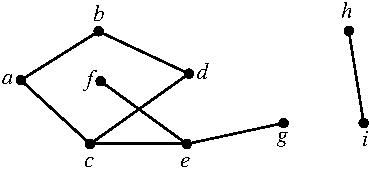
\includegraphics[height=1.5in]{graph-example}
\caption{An example of a graph with 9 nodes and 8 edges.}
\label{fig:graph-example}
\end{figure}

Graphs are ubiquitous in computer science because they provide a handy
way to represent a relationship between pairs of objects;  the objects
represent items of interest such as programs, people, cities, or web
pages, and we place an edge between a pair of nodes if they are
related in a certain way.  For example, an edge between a pair of
people might indicate that they like (or, in alternate scenarios, that
they don't like) each other.  An edge between a pair of courses might
indicate that one needs to be taken before the other.

In this chapter, we will focus our attention on simples graphs where
the relationship denoted by an edge is symmetric.  Afterward, in
Chapter~\ref{chap:digraphs}, we consider the situation where th edge
denotes a one-way relationship (\eg where one web page points to the
other\footnote{Two Stanford students analyzed such a graph to become
  multibillionaires.  So, pay attention to graph theory, and who knows
  what might happen!}).


\section{Definitions}\label{degreessec}

\begin{definition}\label{graphdef}
A \term{simple graph}, $G$, consists of a nonempty set,~$V$, called
the \term{vertices} (aka \emph{nodes}\footnote{We will use the terms
  vertex and node interchangeably.}) of~$G$, and a set, $E$, of
two-element subsets of $V$.  The members of $E$ are called the
\term{edges} of $G$, and we write $G = (V, E)$.
\end{definition}
The vertices correspond to the dots in Figure~\ref{fig:graph-example},
and the edges correspond to the lines.  The graph in
Figure~\ref{fig:graph-example} is expressed mathematically as $G = (V,
E)$, where:
\begin{align*}
V & =  \set{A, B, C, D, E, F, G, H, I} \\
E & =  \set{ \set{A, B}, \set{A, C}, \set{B, D}, \set{C, D},
              \set{C, E}, \set{E, F}, \set{E, G}, \set{H, I} }.
\end{align*}
It will often be helpful to use the notation $\edge{A}{B}$ for the
edge $\set{A,B}$.  Note that $\edge{A}{B}$ and $\edge{B}{A}$ are
different descriptions of the same edge, since sets are unordered.  In
this case, the graph $G = (V, E)$ has 9~nodes and 8~edges

\begin{definition}
Two vertices in a simple graph are said to be \term{adjacent} if they are
joined by an edge, and an edge is said to be \term{incident} to the
vertices it joins.  The number of edges incident to a vertex~$v$ is called the
\term{degree} of the vertex and is denoted by $\degr{v}$;
equivalently, the degree of a vertex is
equals the number of vertices adjacent to it.
\end{definition}
For example, in the simple graph above, $A$ is adjacent to $B$ and $B$
is adjacent to $D$, and the edge $\edge{A}{C}$ is incident to vertices
$A$ and $C$.  Vertex $H$ has degree~1, $D$ has degree~2, and $\degr{E}
= 3$.  It is possible for a vertex to have degree~0, in which case it
is not adjacent to any other vertices.  A simple graph does not need
to have any edges at all (in which case, the degree of every vertex is
zero and $|E| = 0$)\footnote{Recall that the notation $|E|$ denotes the
  cardinality of the set~$E$ (\ie the number of elements of~$E$).},
but it does need to have at least one vertex (\ie $|V| \ge 1$).

Note that simple graphs do \emph{not} have any \emph{self-loops} (\ie
an edge of the form $\{a, a\}$) since an edge is defined to be a set
of \emph{two} vertices.  In addition, there is at most one edge
between any pair of vertices in a simple graph.  In other words, a
simple graph does not contain \emph{multiedges} or \emph{multiple
  edges}.  That is because $E$ is a set.  Lastly, and most
importantly, simple graphs do not contain \emph{directed edges} (\ie
edges of the form~$(a, b)$ instead of~$\{a, b\}$.

There's no harm in relaxing these conditions, and some authors do, but
we don't need self-loops, multiple edges between the same two
vertices, or graphs with no vertices, and it's simpler not to have
them around.  We will consider graphs with directed edges (called
\emph{directed graphs} or \emph{digraphs} at length in
Chapter~\ref{chap:digraphs}.  Since we'll only be considered simple
graphs in this chapter, we'll just call them ``graphs'' from now on.


\subsection{Some Common Graphs}

Some graphs come up so frequently that they have names.  The
\term{complete graph} on $n$ vertices, also called \term{$K_n$}, has
an edge between every two vertices.  For example, $K_5$ is shown in
Figure~\ref{fig:K_5}.

\begin{figure}[h]
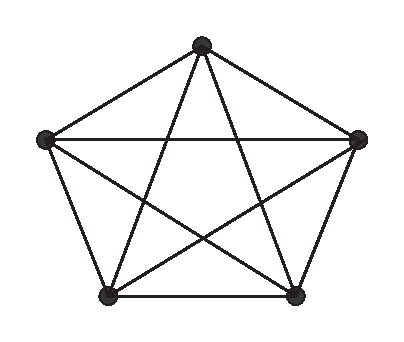
\includegraphics[height=1.5in]{complete-graph}
\caption{The complete graph on 5 nodes, $K_5$.}
\label{fig:K_5}
\end{figure}

The \term{empty graph} has no edges at all.  For example, the empty
graph with 5 nodes is shown in Figure~\ref{fig:graph_empty_5}.

\begin{figure}[h]
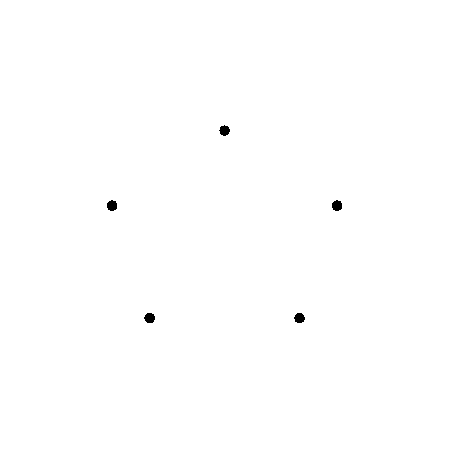
\includegraphics[height=1.5in]{empty-graph}
\caption{The empty graph with 5 nodes.}
\label{fig:graph_empty_5}
\end{figure}

The $n$-node graph containing $n - 1$ edges in sequence is known as
the \emph{line graph}~$L_n$.  More formally, $L_n = (V, E)$ where
\begin{equation*}
    V = \{ v_1, v_2, \dots, v_n \}
\end{equation*}
and
\begin{equation*}
    E = \{\, \{ v_1, v_2 \}, \{ v_2, v_3 \}, \dots, \{ v_{n-1}, v_n \} \,\}
\end{equation*}
For example, $L_5$ is displayed in Figure~\ref{fig:graph_L_5}.

\begin{figure}[h]
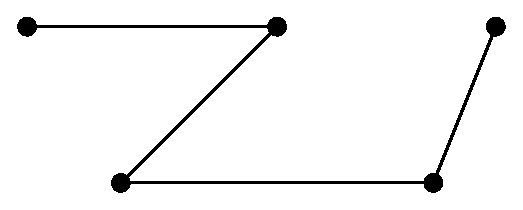
\includegraphics[height=1in]{path-graph}
\caption{The 5-node line graph~$L_5$.}
\label{fig:graph_L_5}
\end{figure}

If we add the edge $\{v_n, v_1\}$ to the line graph~$L_n$, we get the
graph $C_n$ consisting of a simple cycle.  For example, $C_5$ is
illustrated in Figure~\ref{fig:graph_C_5}.

\begin{figure}[h]
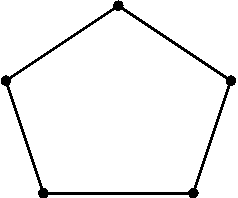
\includegraphics[height=1.5in]{cycle}
\caption{The 5-node cycle graph~$C_5$.}
\label{fig:graph_C_5}
\end{figure}

\subsection{Isomorphism}

Two graphs that look the same might actually be different in a formal
sense.  For example, the two graphs in Figure~\ref{fig:isomorphism}
are both simple cycles with 4~vertices, but one graph has vertex set
$\set{A, B, C, D}$ while the other has vertex set $\set{1, 2, 3, 4}$.
Strictly speaking, these graphs are different mathematical objects,
but this is a frustrating distinction since the graphs \emph{look the
same}!

\begin{figure}
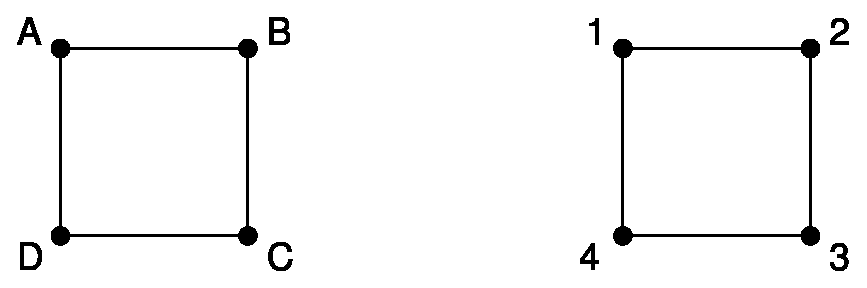
\includegraphics[height=1.5in]{isomorphism}

\textbf{dmj: Add (a) and (b) sublabels}

\caption{Two graphs that are isomorphic to~$C_4$.}
\label{fig:isomorphism}
\end{figure}

Fortunately, we can neatly capture the idea of ``looks the same''
through the notion of graph isomorphism.

\begin{definition}\label{simple-isomorphism}
If $G_1 = (V_1, E_1)$ and $G_2 = (V_2, E_2)$ are two graphs, then we
say that $G_1$ is \term{isomorphic} to $G_2$ iff there exists a
\textbf{bijection}\footnote{A bijection $f: V_1 \to V_2$ is a function
  that associates every node in~$V_1$ with a unique node in~$V_2$ and
  vice-versa.  We will study bijections more deeply in
  Part~\ref{part:counting}.} $f: V_1 \to V_2$ such that for every pair
of vertices $u, v \in V_1$:
\[
\edge{u}{v} \in E_1 \qiff \edge{f(u)}{f(v)} \in E_2.
\]
The function $f$ is called an \term{isomorphism} between $G_1$ and $G_2$.
\end{definition}

In other words, two graphs are isomorphic if they are the same up to a
relabeling of their vertices.
For example, here is an isomorphism between vertices in the two graphs
shown in Figure~\ref{fig:isomorphism}:
\[
\begin{array}{lll}
A \text{ corresponds to } 1 & \hspace{0.5in} & B \text{ corresponds to } 2 \\
D \text{ corresponds to } 4 & & C \text{ corresponds to } 3.
\end{array}
\]
You can check that there is an edge between two vertices in the graph
on the left if and only if there is an edge between the two
corresponding vertices in the graph on the right.

Two isomorphic graphs may be drawn very differently.  For example, we
have shown two different ways of drawing $C_5$ in
Figure~\ref{fig:isomorphism-c5}.

\begin{figure}[h]
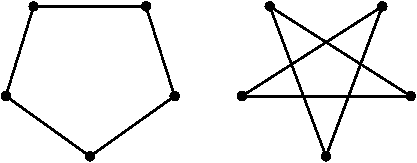
\includegraphics[height=1.5in]{isomorphism-c5}
\caption{Two ways of drawing $C_5$.}
\label{fig:isomorphism-c5}
\end{figure}

Isomorphism preserves the connection properties of a graph,
abstracting out what the vertices are called, what they are made out
of, or where they appear in a drawing of the graph.  More precisely, a
property of a graph is said to be \term{preserved under isomorphism}
if whenever $G$ has that property, every graph isomorphic to $G$ also
has that property.  For example, isomorphic graphs must have the same
number of vertices.  What's more, if $f$ is a graph isomorphism that
maps a vertex, $v$, of one graph to the vertex, $f(v)$, of an
isomorphic graph, then by definition of isomorphism, every vertex
adjacent to $v$ in the first graph will be mapped by $f$ to a vertex
adjacent to $f(v)$ in the isomorphic graph.  That is, $v$ and $f(v)$
will have the same degree.  So if one graph has a vertex of degree 4
and another does not, then they can't be isomorphic.  In fact, they
can't be isomorphic if the number of degree 4 vertices in each of the
graphs is not the same.

Looking for preserved properties can make it easy to determine that
two graphs are not isomorphic, or to actually find an isomorphism
between them if there is one.  In practice, it's frequently easy to
decide whether two graphs are isomorphic.  However, no one has yet
found a
\emph{general} procedure for determining whether two graphs are isomorphic
that is \emph{guaranteed} to run in polynomial
time\footnote{\emph{I.e.}, in an amount of time that is upper-bounded
  by $|V|^c$ where $c$ is a fixed number independent of~$|V|$.}
in~$|V|$.

Having an efficient procedure to detect isomorphic graphs would, for
example, make it easy to search for a particular molecule in a database
given the molecular bonds.  On the other hand, knowing there is no such
efficient procedure would also be valuable: secure protocols for
encryption and remote authentication can be built on the hypothesis that
graph isomorphism is computationally exhausting.

\subsection{Subgraphs}

\begin{definition}\label{def:subgraph}
A graph $G_1 = (V_1, E_1)$ is said to be a \emph{subgraph} of a graph
$G_2 = (V_2, E_2)$ if
$V_1 \subseteq V_2$ and $E_1 \subseteq E_2$.
\end{definition}

For example, the empty graph on $n$ nodes is a subgraph of~$L_n$,
\ $L_n$ is a subgraph of~$C_n$, and $C_n$ is a subgraph of~$K_n$.
Also, the graph $G = (V, E)$ where
\begin{equation*}
    V = \{ G, H, I \} and E = \{\, \{ H, I \} \,\}
\end{equation*}
is a subgraph of the graph in Figure~\ref{fig:graph-example}.  On the
other hand, any graph containing an edge~$\{G, H\}$ would not be a
subgraph of the graph in Figure~\ref{fig:graph-example} because the
graph in Figure~\ref{fig:graph-example} does not contain this edge.

Note that since a subgraph is itself a graph, the endpoints of any
edge in a subgraph must also be in the subgraph.  In other words if
$G' = (V', E')$ is a subgraph of some graph~$G$, and $\{ v_i, v_j \}
\in E'$, then it must be the case that $v_i \in V'$ and $v_j \in V'$.

\subsection{Weighted Graphs}

Sometimes, we will use edges to denote a connection between a pair of
nodes where the connection has a \emph{capacity} or \emph{weight}.
For example, we might be interested in the capacity of an internet
fiber between a pair of computers, the resistance of a wire between a
pair of terminals, the tension of a spring connecting a pair of
devices in a dynamical system, the tension of a bond between a pair of
atoms in a molecule, or the distance of a highway betwen a pair of
citis.

In such cases, it is useful to represent the system with an
\emph{edge-weighted} graph (aka a \emph{weighted graph}).  A weighted
graph is the same as a simple graph except that we associate a real
number (\ie the weight) with each edge in the graph.  Mathematically
speaking, a weighted graph consists of a graph $G = (V, E)$ and a
weight function $w: E \to \reals$.  For example,
Figure~\ref{fig:weighted_graph} shows a weighted graph where the
weight of edge $\edge{A}{B}$ is~5.

\begin{figure}
\textbf{dmj: make figure}

\caption{A 4-node weighted graph where an edge~$\edge{A}{B}$ has
  weight~5.}
\label{fig:weighted_graph}
\end{figure}

\subsection{Adjacency Matrices}

There are many ways to represent a graph.  We have already seen two
ways: you can draw it (\eg as in Figure~\ref{fig:weighted_graph}), and
you can represent it with sets (as in $G = (V, E)$).  Another common
representation is with an adjacency matrix.

\begin{definition}\label{def:adjacency_matrix}

Given an $n$-node graph $G = (V, E)$ where $V = \{ v_1, v_2, \dots,
v_n \}$, the \term{adjacency matrix} for~$G$ is the $n \by n$ matrix
$A_G = \{ a_{ij} \}$ where
\begin{equation*}
    a_{ij} = \begin{cases}
                1 & \text{if $\{ v_i, v_j \} \in E$} \\
                0 & \text{otherwise.}
              \end{cases}
\end{equation*}
If $G$ is a weighted graph with edge weight given by $w: E \to
\reals$, then the adjacency matrix for~$G$ is $A_G = \{ a_{ij} \}$
where
\begin{equation*}
    a_{ij} = \begin{cases}
                w(\{ v_i, v_j \}) & \text{if $\{ v_i, v_j \} \in E$} \\
                0                 & \text{otherwise.}
              \end{cases}
\end{equation*}
\end{definition}

For example, Figure~\ref{fig:adjacency_matrix} displays the adjacency
matrices for the graphs shown in Figures~\ref{fig:isomorphism}(a)
and~\ref{fig:weighted_graph} where $v_1 = A$, $v_2 = B$, $v_3 = C$,
and $v_4 = D$.

\begin{figure}[h]

\subfloat[]{%
    $
       \begin{pmatrix}
           0 & 1 & 0 & 1 \\
           1 & 0 & 1 & 0 \\
           0 & 1 & 0 & 1 \\
           1 & 0 & 1 & 0
       \end{pmatrix}
   $
}
\qquad
\subfloat[]{%
   $
       \begin{pmatrix}
           0 & 5 & 0 & 0 \\
           5 & 0 & 6 & 0 \\
           0 & 6 & 0 & -3 \\
           0 & 0 & -3 & 0
       \end{pmatrix}
   $
}

\caption{Examples of adjacency matrices.  (a)~shows the adjacency
  matrix for the graph in Figure~\ref{fig:isomorphism}(a) and
  (b)~shows the adjacency matrix for the weighted graph in
  Figure~\ref{fig:weighted_graph}.  In each case, we use the set $v_1
  = A$, $v_2 = B$, $v_3 = C$, and $v_4 = D$ to construct the matrix.}
\label{fig:adjacency_matrix}
\end{figure}

%% Simple Graphs Problems %%%%%%%%%%%%%%%%%%%%%%%%%%%%%%%%%%%%%%%%%%%%%%%%%%%%%
\begin{problems}
\classproblems
\pinput{CP_Handshaking_Lemma}
\pinput{CP_isomorphic_graphs}
% S09.cp6m.1
% S09.cp6m.3
% S09.cp6m.4

\homeworkproblems
\pinput{PS_choose_isomorphic_graphs}
\pinput{PS_neighbors_under_isomorphisms}
\pinput{PS_graph_two_ends}

\examproblems
\pinput{MQ_list_isomorphisms}
\pinput{FP_bipartite_matching_sex}
\end{problems}


\section{Matching Problems}

We begin our study of graph theory by considering the scenario where
the nodes in a graph represent people and edges represent a
relationship between pairs of people such as ``likes'', ``marries'',
and so on.  Now, you may be wondering what marriage has to do with
computer science, and with good reason.  It turns out that the
techniques we will develop apply to much more general scenarios where
instead of matching men to women, we need to match packets to paths in
a network, applicants to jobs, or internet traffice to webservers.

In our first example, we will show how graph theory can be used to
debunk an urban legend about sexual practices in America.  Yes, you
read correctly.  So, fasten your seat belt---who knew that math might
actually be interesting!

\subsection{Sex in America}

On average, who has more opposite-gender partners: men or women?

Sexual demographics have been the subject of many studies.  In one of the
largest, researchers from the University of Chicago interviewed a random
sample of 2500 Americans over several years to try to get an answer to this
question.  Their study, published in 1994, and entitled \emph{The Social
  Organization of Sexuality} found that on average men have 74\% more
opposite-gender partners than women.

Other studies have found that the disparity is even larger.  In
particular, ABC News claimed that the average man has 20 partners over his
lifetime, and the average woman has 6, for a percentage disparity of
233\%.  The ABC News study, aired on Primetime Live in 2004, purported to
be one of the most scientific ever done, with only a 2.5\% margin of
error.  It was called "American Sex Survey: A peek between the sheets."
The promotion for the study is even better:
\begin{quote}
``A ground breaking ABC News `Primetime Live' survey finds a range of
eye-popping sexual activities, fantasies and attitudes in this country,
confirming some conventional wisdom, exploding some myths----and venturing
where few scientific surveys have gone before.''
\end{quote}
Probably that last part about going where few scientific surveys have gone
before is pretty accurate!

Yet again, in August, 2007, the N.Y. Times reported
%% \href{The-Myth-the-Math-the-Sex.pdf}{reported}
%% \iffalse
%% \href{http://www.nytimes.com/2007/08/12/weekinreview/12kolata.html?_r=1&n=Top/Reference/Times%20Topics/People/K/Kolata,%20Gina&oref=slogin}{reported}
%% \fi
on a study by the National Center for Health Statistics of the
U.S. Government showing that men had seven partners while women had
four.

Anyway, whose numbers do you think are more accurate, the University
of Chicago, ABC News, or the National Center for Health
Statistics?---don't answer; this is a setup question like ``When did
you stop beating your wife?''  Using a little graph theory, we will
now explain why none of these findings can be anywhere near the truth.

Let's model the question of heterosexual partners in graph theoretic
terms.  To do this, we'll let $G$ be the graph whose vertices, $V$,
are all the people in America.  Then we split $V$ into two separate
subsets: $M$, which contains all the males, and $F$, which contains
all the females.\footnote{For simplicity, we'll ignore the possibility
  of someone being both, or neither, a man and a woman.}  We'll put an
edge between a male and a female iff they have been sexual partners.
A possible subgraph of this graph is illustrated in
Figure~\ref{fig:partners} with males on the left and females on the
right.

\begin{figure}[htbp]
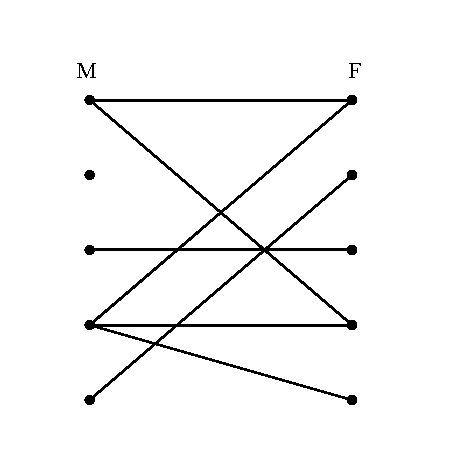
\includegraphics[height=1.75in]{sex-edges}
\caption{The sex partners graph}
\label{fig:partners}
\end{figure}

Actually, $G$ is a pretty hard graph to figure out, let alone draw.
The graph is \emph{enormous}: the US population is about 300 million,
so $\card{V} \approx 300M$.  In the United States, approximately
50.8\% of the populatin is female and 49.2\% is male, and so $\card{M}
\approx 147.6M$, and $\card{F} \approx 152.4M$.  And we don't even
have trustworthy estimates of how many edges there are, let alone
exactly which couples are adjacent.  But it turns out that we don't
need to know any of this to debunk the sex surveys---we just need to
figure out the relationship between the average number of partners per
male and partners per female.  To do this, we note that every edge is
incident to exactly one $M$ vertex and one $F$ vertex (remember, we're
only considering male-female relationships); so the sum of the degrees
of the $M$ vertices equals the number of edges, and the sum of the
degrees of the $F$ vertices equals the number of edges.  So these sums
are equal:
%
\[
\sum_{x \in M} \degr{x} = \sum_{y \in F} \degr{y}.
\]
%
If we divide both sides of this equation by the product of the sizes
of the two sets, $\card{M} \cdot \card{F}$, we obtain
%
\begin{equation}\label{eq:average-degree}
\left(\frac{\sum_{x \in M} \degr{x}}{\card{M}}\right) \cdot \frac{1}{\card{F}} =
\left(\frac{\sum_{y \in F} \degr{y}}{\card{F}}\right) \cdot \frac{1}{\card{M}}
\end{equation}
Notice that
\begin{equation*}
    \frac{\sum_{x \in M} \degr{x}}{\card{M}}
\end{equation*}
is simply the average degree of a node in~$M$.  This is the average
number of opposite-gender partners for a male in America.  Similarly,
\begin{equation*}
    \frac{\sum_{x \in F} \degr{x}}{\card{F}}
\end{equation*}
is the average degree of a node in~$F$, which is the average number of
opposite-gender partners for a female in America.  Hence,
Equation~\ref{eq:average-degree} implies that on average, an American
male has $|F|/|M|$ times as many opposite-gender partners as the
average American female.

From the Census Bureau reports, we know that there are slightly more
females than males in America; in particular $\card{F} / \card{M}$ is
about 1.035.  So we know that on average, males have 3.5\% more
opposite-gender partners than females.  Of course, this statistic
really says nothing about
any sex's promiscuity or selectivity.  Remarkably, promiscuity is
completely irrelevant in this analysis.  That is because the ration of
the average number of partners is completely determined by the
relative number of males and females.  Collectively, males and
females have the same number of opposite gender partners, since it
takes one of each set for every partnership, but there are fewer
males, so they have a higher ratio.  This means that the University of
Chicago, ABC, and the Federal Government studies are way off.  After a
huge effort, they gave a totally wrong answer.

There's no definite explanation for why such surveys are consistently wrong.  One
hypothesis is that males exaggerate their number of partners ---or maybe females
downplay theirs ---but these explanations are speculative.  Interestingly, the
principal author of the National Center for Health Statistics study reported that she
knew the results had to be wrong, but that was the data collected, and her job was to
report it.

The same underlying issue has led to serious misinterpretations of other survey data.
For example, a few years ago, the Boston Globe ran a story on a survey of the
study habits of students on Boston area campuses.  Their survey showed that on average,
minority students tended to study with non-minority students more than the other way
around.  They went on at great length to explain why this ``remarkable phenomenon''
might be true.  But it's not remarkable at all ---using our graph theory formulation,
we can see that all it says is that there are fewer minority students than non-minority
students, which is, of course what ``minority'' means.

\subsubsection{The Handshaking Lemma}

The previous argument hinged on the connection between a sum of
degrees and the number edges.  There is a simple connection between
these quantities in any graph:
\begin{lemma}\label{sumedges}
The sum of the degrees of the vertices in a graph equals twice the number of edges.
\end{lemma}

\begin{proof}
Every edge contributes two to the sum of the degrees, one for each of its endpoints.
\end{proof}

Lemma~\ref{sumedges} is sometimes called the \term{Handshake Lemma}:
if we total up the number of people each person at a party shakes
hands with, the total will be twice the number of handshakes that
occurred.

%% INSERT H GOES HERE

\subsection{The Stable Marriage Problem}
\label{stablemarriagesec}

\providecommand{\boys}{\text{the-Boys}}
\providecommand{\girls}{\text{the-Girls}}
\providecommand{\qst}{\text{$q_0$}}
\providecommand{\none}{\texttt{none}}
\providecommand{\girln}{\text{$\girls \union \set{\none}$}}
\providecommand{\boyn}{\text{$\boys \union \set{\none}$}}
\providecommand{\sere}{\text{\emph{serenading}}}
\providecommand{\suit}{\text{\emph{suitors}}}
\providecommand{\fav}{\text{\emph{favorite}}}
\providecommand{\nex}{\text{\emph{next}}}
\providecommand{\tgn}{\text{\emph{total-girls-names}}}

\subsubsection{The Problem}

We next consider a version of the bipartite matching problem where
there are an equal number of men and women, and where each person has
preferences about who they would like to marry.  In fact, we assume
that each man he has a complete list of all the women ranked according
to his preferences, with no ties.  Likewise, each woman has a ranked
list of all of the men.

The preferences don't have to be symmetric.  That is, Jennifer might
like Brad best, but Brad doesn't necessarily like Jennifer best.  The
goal is to marry everyone: every man must marry exactly one woman and
vice-versa---no polygamy.  Moreover, we would like to find a matching
between men and women that is \emph{stable} in the sense that there is
no pair of people that prefer each other to their spouses.

For example, suppose \emph{every} man likes Angelina best, and every
woman likes Brad best, but Brad and Angelina are married to other
people, say Jennifer and Billy Bob.  Now \emph{Brad and Angelina
  prefer each other to their spouses}, which puts their marriages at
risk: pretty soon, they're likely to start spending late nights
together working on problem sets!

This unfortunate situation is illustrated in
Figure~\ref{fig:minWtMatch2}, where the digits ``1'' and ``2'' near a
man shows which of the two women he ranks first second, respectively,
and similarly for the women.

\begin{figure}[h]
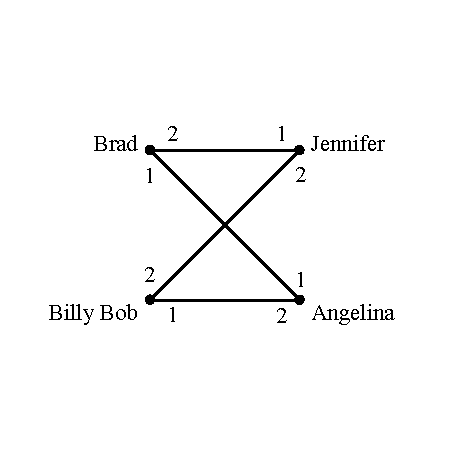
\includegraphics[height=1.2in]{minWtMatch2}

\caption{Preferences for four people.  Both men like Angelina best and
both women like Brad best.}
\label{fig:minWtMatch2}
\end{figure}

More generally, in any matching, a man and woman who are not married
to each other and who like each other better than their spouses, is
called a \emph{rogue couple}.  In the situation shown in
Figure~\ref{fig:minWtMatch2}, Brad and Angelina would be a rogue
couple.

Having a rogue couple is not a good thing, since it threatens the
stability of the marriages.  On the other hand, if there are no rogue
couples, then for any man and woman who are not married to each other,
at least one likes their spouse better than the other, and so they
won't be tempted to start an affair.

\begin{definition}
  A \term{stable matching} is a matching with no rogue couples.
\end{definition}

The question is, given everybody's preferences, how do you find a
stable set of marriages?  In the example consisting solely of the four
people in Figure~\ref{fig:minWtMatch2}, we could let Brad and Angelina
both have their first choices by marrying each other.  Now neither
Brad nor Angelina prefers anybody else to their spouse, so neither
will be in a rogue couple.  This leaves Jen not-so-happily married to
Billy Bob, but neither Jen nor Billy Bob can entice somebody else to
marry them, and so there is a stable matching.

It is something of a surprise that there always is a stable matching
among a group of men and women, and we'll shortly explain why.  The
surprise springs in part from considering the apparently similar
``buddy'' matching problem.  That is, if people can be paired off as
buddies, regardless of gender, then a stable matching \emph{may not}
be possible.  For example, Figure~\ref{fig:buddy} shows a situation
with a love triangle and a fourth person who is everyone's last
choice.  In this figure Mergatoid's preferences aren't shown because
they don't even matter.

\begin{figure}[htbp]
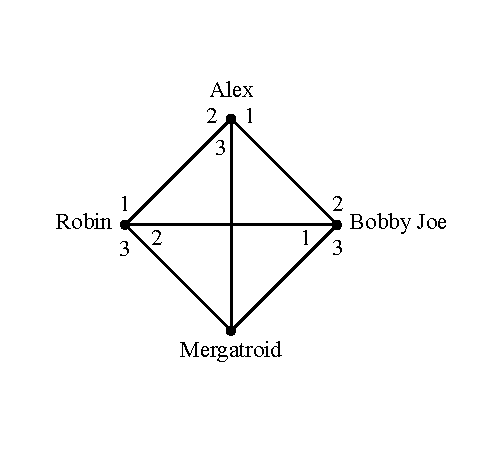
\includegraphics[height=2.3in]{loveTriangle}
\caption{Some preferences with no stable buddy matching.}
\label{fig:buddy}
\end{figure}

Let's see why there is no stable matching:
\begin{lemma}\label{lem:nostablematch}
There is no stable buddy matching among the four people in
Figure~\ref{fig:buddy}.
\end{lemma}

\begin{proof}
We'll prove this by contradiction.

Assume, for the purposes of contradiction, that there is a stable
matching.  Then there are two members of the love triangle that are
matched.  Since preferences in the triangle are symmetric, we may assume
in particular, that Robin and Alex are matched.  Then the other pair must
be Bobby-Joe matched with Mergatoid.

But then there is a rogue couple: Alex likes Bobby-Joe best, and Bobby-Joe
prefers Alex to his buddy Mergatoid.  That is, Alex and Bobby-Joe are a
rogue couple, contradicting the assumed stability of the matching.
\end{proof}

So getting a stable \emph{buddy} matching may not only be hard, it may
be impossible.  But when mens are only allowed to marry women, and
vice versa, then it turns out that a stable matching can always be
found.\footnote{Once again, we disclaim any political statement
  here---its just the way that the math works out.}

%%insert rest of story from gusfield book pp3--4??

\iffalse

\subsection{Failed attempts}

Let's find a stable matching in one possible situation, and hope to
translate our method to a general algorithm.  The table below shows the
preferences of each girl and boy in decreasing order.

\begin{eqnarray*}
boys & \quad & girls \\
1 : C B E A D & \quad & A : 3 5 2 1 4 \\
2 : A B E C D & \quad & B : 5 2 1 4 3 \\
3 : D C B A E & \quad & C : 4 3 5 1 2 \\
4 : A C D B E & \quad & D : 1 2 3 4 5 \\
5 : A B D E C & \quad & E : 2 3 4 1 5
\end{eqnarray*}

How about we try a ``greedy'' strategy?\footnote{``Greedy'' is not any
moral judgment.  It refers to algorithms that work by always choosing the
next state that makes the largest immediate progress.}  We simply take
each boy in turn and pack him off with his favorite among the girls still
available.  This gives the following assignment.

\begin{eqnarray*}
1 \rightarrow C \\
2 \rightarrow A \\
3 \rightarrow D \\
4 \rightarrow B \\
5 \rightarrow E \\
\end{eqnarray*}

To determine whether this matching is stable, we have to check whether
there are any rogue couples.  Boys 1, 2, and 3 all got their top pick
among the girls; none would even think of running off.  Boy 4 may be a
problem because he likes girl $A$ better than his mate, but she ranks him
dead last.  However, boy 4 also likes girl $C$ better than his mate, and
she rates him above her own mate.  Therefore, boy 4 and girl $C$ form a
rogue couple!  The marriages are not stable.  We could try to make ad hoc
repairs, but we're really trying to develop a general strategy.

Another approach would be to use induction.  Suppose we pair Boy 1 with
his favorite girl, $C$, try to show that neither of these two will be
involved in a rogue couple, and then solve the remaining problem by
induction.  Clearly Boy 1 will never leave his top pick, Girl $C$.  But
the problem with this approach is that we \emph{can't} be sure that Girl
$C$ won't be in a rogue couple.  Girl $C$ might very well dump Boy 1 --
she might even rate him last!

This turns out to be a tricky problem.  The best approach is to use a
mating ritual that is reputed to have been popular in some mythic past.
\fi

\subsubsection{The Mating Ritual}

The procedure for finding a stable matching involves a \emph{Mating
Ritual} that takes place over several days.  The following events happen
each day:

\textbf{Morning}: Each girl stands on her balcony.  Each boy stands under
the balcony of his favorite among the girls on his list, and he serenades
her.  If a boy has no girls left on his list, he stays home and does his
6.042 homework.

\textbf{Afternoon}: Each girl who has one or more suitors serenading
her, says to her favorite among them, ``We might get engaged.  Come
back tomorrow.''  To the other suitors, she says, ``No.  I will never
marry you!  Take a hike!''

\textbf{Evening}: Any boy who is told by a girl to take a hike, crosses that
girl off his list.

\textbf{Termination condition}: When every girl has at most one suitor,
the ritual ends with each girl marrying her suitor, if she has one.

% Show example

There are a number of facts about this Mating Ritual that we would like to
prove:

\begin{itemize}
\item The Ritual has a last day.
\item Everybody ends up married.
\item The resulting marriages are stable.
\end{itemize}

\subsection{A State Machine Model}

Before we can prove anything, we should have clear mathematical
definitions of what we're talking about.  In this section we sketch how to
define a rigorous state machine model of the Marriage Problem.

So let's begin by formally defining the problem.

\begin{definition}
  A \term{Marriage Problem} consists of two disjoint sets of the same
  finite size, called \boys\ and \girls.  The members of \boys\ are called
  \emph{boys}, and members of \girls\ are called \emph{girls}.  For each
  boy, $B$, there is a strict total order, \term{$<_B$}, on \girls, and
  for each girl, $G$, there is a strict total order, \term{$<_G$}, on
  \boys.  If $G_1 <_B G_2$ we say $B$ \term*{prefers} girl $G_2$ to girl
  $G_1$.  Similarly, if $B_1 <_G B_2$ we say $G$ \term{prefers} boy $B_2$
  to boy $B_1$.

A \term{marriage assignment} or \term{perfect matching} is a bijection,
$w:\boys \to \girls$.  If $B \in \boys$, then $w(B)$ is called $B$'s
\emph{wife} in the assignment, and if $G \in \girls$, then $w^{-1}(G)$ is
called $G$'s \emph{husband}.  A \term{rogue couple} is a boy, $B$, and a
girl, $G$, such that $B$ prefers $G$ to his wife, and $G$ prefers $B$ to
her husband.  An assignment is \term{stable} if it has no rogue couples.
A \term{solution} to a marriage problem is a stable perfect matching.
\end{definition}

To model the Mating Ritual with a state machine, we make a key
observation: to determine what happens on any day of the Ritual, all we
need to know is which girls are still on which boys' lists on the morning of
that day.  So we define a state to be some mathematical data structure
providing this information.  For example, we could define a state to be
the ``still-has-on-his-list'' relation, $R$, between boys and girls, where
$B\mrel{R}G$ means girl $G$ is still on boy $B$'s list.

We start the Mating Ritual with no girls crossed off.  That is, the start
state is the \emph{\idx{complete bipartite}} relation in which every boy
is related to every girl.

According to the Mating Ritual, on any given morning, a boy will
\term{serenade} the girl he most prefers among those he has not as yet
crossed out.  Mathematically, the girl he is serenading is just the
maximum among the girls on $B$'s list, ordered by $<_B$.  (If the list is
empty, he's not serenading anybody.)  A girl's \term{favorite} is just the
maximum, under her preference ordering, among the boys serenading her.

Continuing in this way, we could mathematically specify a precise Mating
Ritual state machine, but we won't bother.  The intended behavior of the
Mating Ritual is clear enough that we don't gain much by giving a formal
state machine, so we stick to a more memorable description in terms of
boys, girls, and their preferences.  The point is, though, that it's not
hard to define everything using basic mathematical data structures like
sets, functions, and relations, if need be.

\subsection{There is a Marriage Day}

It's easy to see why the Mating Ritual has a terminal day when people
finally get married.  Every day on which the ritual hasn't terminated, at
least one boy crosses a girl off his list.  (If the ritual hasn't
terminated, there must be some girl serenaded by at least two boys, and at
least one of them will have to cross her off his list).  So starting with
$n$ boys and $n$ girls, each of the $n$ boys' lists initially has $n$
girls on it, for a total of $n^2$ list entries.  Since no girl ever gets
added to a list, the total number of entries on the lists decreases every
day that the Ritual continues, and so the Ritual can continue for at most
$n^2$ days.

\subsection{They All Live Happily Every After...}

We still have to prove that the Mating Ritual leaves everyone in a
stable marriage.  To do this, we note one very useful fact about the
Ritual: if a girl has a favorite boy suitor on some morning of the Ritual,
then that favorite suitor will still be serenading her the next morning
---because his list won't have changed.  So she is sure to have today's
favorite boy among her suitors tomorrow.  That means she will be able to
choose a favorite suitor tomorrow who is at least as desirable to her as
today's favorite.  So day by day, her favorite suitor can stay the same or
get better, never worse.  In others words, a girl's favorite is a weakly
increasing variable with respect to her preference order on the boys.

Now we can verify the Mating Ritual using a simple invariant predicate,
$P$, that captures what's going on:
\begin{quotation}
  For every girl, $G$, and every boy, $B$, if $G$ is crossed off $B$'s
  list, then $G$ has a suitor whom she prefers over $B$.
\end{quotation}

Why is $P$ invariant?  Well, we know that $G$'s favorite tomorrow will be
at least as desirable to her as her favorite today, and since her favorite
today is more desirable than $B$, tomorrow's favorite will be too.

Notice that $P$ also holds on the first day, since every girl is on every
list.  So by the Invariant Theorem, we know that $P$ holds on every day
that the Mating Ritual runs.  Knowing the invariant holds when the
Mating Ritual terminates will let us complete the proofs.

\begin{theorem}
Everyone is married by the Mating Ritual.
\end{theorem}

\begin{proof}
  Suppose, for the sake of contradiction, that it is the last day of
  the Mating Ritual and some boy does not get married.  Then he can't
  be serenading anybody, and so his list must be empty.  So by invariant
  $P$, every girl has a favorite boy whom she prefers to that boy.  In
  particular, every girl has a favorite boy whom she marries on the
  last day.  So all the girls are married.  What's more there is no
  bigamy: a boy only serenades one girl, so no two girls have the same
  favorite.

But there are the same number of girls as boys, so all the boys must be
married too.
\end{proof}

\begin{theorem}
The Mating Ritual produces a stable matching.
\end{theorem}

\begin{proof}
Let Brad be some boy and Jen be any girl that he is \emph{not} married to
on the last day of the Mating Ritual.  We claim that Brad and Jen are not
a rogue couple.  Since Brad is an arbitrary boy, it follows that no boy is
part of a rogue couple.  Hence the marriages on the last day are stable.

To prove the claim, we consider two cases:

\emph{Case} 1.  Jen is not on Brad's list.  Then by invariant $P$, we know
that Jen prefers her husband to Brad.  So she's not going to run off with
Brad: the claim holds in this case.

\emph{Case} 2.  Otherwise, Jen is on Brad's list.  But since Brad is not
married to Jen, he must be choosing to serenade his wife instead of Jen,
so he must prefer his wife.  So he's not going to run off with Jen: the
claim also holds in this case.
\end{proof}


\subsection{...Especially the Boys}

Who is favored by the Mating Ritual, the boys or the girls?  The girls
seem to have all the power: they stand on their balconies choosing the
finest among their suitors and spurning the rest.  What's more, we know
their suitors can only change for the better as the Ritual progresses.
Similarly, a boy keeps serenading the girl he most prefers among those on
his list until he must cross her off, at which point he serenades the next
most preferred girl on his list.  So from the boy's point of view, the
girl he is serenading can only change for the worse.  Sounds like a good
deal for the girls.

But it's not!  The fact is that from the beginning, the boys are
serenading their first choice girl, and the desirability of the girl being
serenaded decreases only enough to give the boy his most desirable
possible spouse.  The mating algorithm actually does as well as possible
for all the boys and does the worst possible job for the girls.

To explain all this we need some definitions.  Let's begin by observing
that while the mating algorithm produces one stable matching, there may be
other stable matchings among the same set of boys and girls.  For example,
reversing the roles of boys and girls will often yield a different stable
matching among them.

But some spouses might be out of the question in all possible stable
matchings.  For example, Brad is just not in the realm of possibility for
Jennifer, since if you ever pair them, Brad and Angelina will form a rogue
couple; here's a picture:

\mfigure{!}{1.2in}{exampleOpt}

\begin{definition}
Given any marriage problem, one person is in another person's \emph{realm
of possible spouses} if there is a stable matching in which the two people
are married.  A person's \term{optimal spouse} is their most preferred
person within their realm of possibility.  A person's \term{pessimal
spouse} is their least preferred person in their realm of possibility.
\end{definition}

Everybody has an optimal and a pessimal spouse, since we know there is at
least one stable matching, namely the one produced by the Mating Ritual.
Now here is the shocking truth about the Mating Ritual:

\begin{theorem}\label{boyopt}
The Mating Ritual marries every boy to his optimal spouse.
\end{theorem}

\begin{proof}
Assume for the purpose of contradiction that some boy does not get his
optimal girl.  There must have been a day when he crossed off his optimal
girl ---otherwise he would still be serenading her or some even more
desirable girl.

By the Well Ordering Principle, there must be a \emph{first} day when a
boy, call him ``Keith,'' crosses off his optimal girl, Nicole.

According to the rules of the Ritual, Keith crosses off Nicole because
Nicole has a favorite suitor, Tom, and
\begin{quote}
Nicole prefers Tom to Keith (*)
\end{quote}
(remember, this is a proof by contradiction \smiley\ ).

Now since this is the first day an optimal girl gets crossed off, we know
Tom hasn't crossed off his optimal girl.  So
\begin{quote}
Tom ranks Nicole at least as high as his optimal girl. (**)
\end{quote}
By the definition of an optimal girl, there must be some stable set of
marriages in which Keith gets his optimal girl, Nicole.  But then the
preferences given in ~(*) and~(**) imply that Nicole and Tom are a
rogue couple within this supposedly stable set of marriages (think
about it).  This is a contradiction.
\end{proof}

\begin{theorem}
The Mating Ritual marries every girl to her pessimal spouse.
\end{theorem}

\begin{proof}
Say Nicole and Keith marry each other as a result of the Mating Ritual.
By the previous Theorem~\ref{boyopt}, Nicole is Keith's optimal spouse,
and so in any stable set of marriages,
\begin{quote}
Keith rates Nicole at least as high as his spouse. (+)
\end{quote}

Now suppose for the purpose of contradiction that there is another stable
set of marriages where Nicole does worse than Keith.  That is, Nicole is
married to Tom, and
\begin{quote}
Nicole prefers Keith to Tom (++)
\end{quote}
Then in this stable set of marriages where Nicole is married to Tom,~(+)
and~(++) imply that Nicole and Keith are a rogue couple, contradicting
stability.  We conclude that Nicole cannot do worse than Keith.
\end{proof}

\subsection{Applications}

Not surprisingly, a stable matching procedure is used by at least one
large dating agency.  But although ``boy-girl-marriage'' terminology is
traditional and makes some of the definitions easier to remember (we hope
without offending anyone), solutions to the Stable Marriage Problem are
widely useful.

The Mating Ritual was first announced in a paper by D. \idx{Gale} and
L.S. \idx{Shapley} in 1962, but ten years before the Gale-Shapley paper was
appeared, and unknown by them, the Ritual was being used to assign
residents to hospitals by the National Resident Matching Program (NRMP).
The NRMP has, since the turn of the twentieth century, assigned each
year's pool of medical school graduates to hospital residencies (formerly
called ``internships'') with hospitals and graduates playing the roles of
boys and girls.  (In this case there may be multiple boys married to one
girl, but there's an easy way to use the Ritual in this situation (see
Problem~\ref{PS_stable_matching_hospitals}).  Before the Ritual was
adopted, there were chronic disruptions and awkward countermeasures taken
to preserve assignments of graduates to residencies.  The Ritual resolved
these problems so successfully, that it was used essentially without
change at least through 1989.\footnote{Much more about the Stable Marriage
  Problem can be found in the very readable mathematical monograph by Dan
  Gusfield and Robert W. Irving,
  \href{http://mitpress.mit.edu/catalog/item/default.asp?ttype=2&tid=7676}{The
    Stable Marriage Problem: Structure and Algorithms}, MIT Press,
  Cambridge, Massachusetts, 1989, 240 pp.}

The internet infrastructure company, Akamai, also uses a variation of
the Gale-Shapley procedure to assign web traffic to servers.  In the
early days, Akamai used other combinatorial optimization algorithms
that got to be too slow as the number of servers (over 20,000 in 2010)
\textcolor{red}{reference needed} and traffic increased.  Akamai switched
to Gale-Shapley since it is fast and can be run in a distributed
manner.  In this case, the web traffic corresponds to the boys and the
web servers to the girls.  The servers have preferences based on
latency and packet loss; the traffic has preferences based on the cost
of bandwidth.

\begin{problems}
\practiceproblems

\pinput{CP_mating_ritual_example}

\pinput{TP_mating_ritual_invariant}

\classproblems

\pinput{CP_mating_ritual_proof}

\pinput{CP_stable_matching_non_optimal}

\homeworkproblems

\pinput{PS_stable_matching_hospitals}

\pinput{PS_stable_matching_no_first_choice}

\pinput{PS_stable_matching_unlucky}

\begin{editingnotes}
Add problem proving that the Mating Ritual need not proceed in
morning/afternoon/evening lock step: a girl can reject nonfavorite
suitors one at a time and at any time, and a rejected boy can change
the girl he serenades without waiting for the other boys to change.
The proof uses the fact that single actions commute, so induction
proves that all executions are confluent ---which implies all
executions end with the same boy-optimal matching.  This lemma can be
cited in the planar graphs section to prove that the edges in an
embedding can be added in any order.
\end{editingnotes}
\end{problems}

%% Connectedness %%%%%%%%%%%%%%%%%%%%%%%%%%%%%%%%%%%%%%%%%%%%%%%%%%%%%%%%%%%%%%

\hyperdef{connect}{edness}{\section{Connectedness}}

\subsection{Paths and Simple Cycles}

\emph{Paths} in simple graphs are esentially the same as paths in digraphs.
We just modify the digraph definitions using undirected edges instead of directed
ones.  For example, the formal definition of a path in a simple graph is a virtually
that same as Definition~\ref{def:digraph-paths} of paths in digraphs:

\begin{definition}\label{def:undirected-path}
A \term{path} in a graph, $G$, is a sequence of $k \geq 0$ vertices
\[
v_0,\dots,v_k
\]
such that $\edge{v_i}{v_{i+1}}$ is an edge of $G$ for all $i$ where $0
\leq i < k$ .  The path is said to \index{start of path}\emph{start} at
$v_0$, to \index{end of path}\emph{end} at $v_k$, and the \index{length of
  path}\emph{length} of the path is defined to be $k$.

An edge, $\edge{u}{v}$, is \term{traversed} $n$ times by the path if there
are $n$ different values of $i$ such that $\edge{v_i}{v_{i+1}} =
\edge{u}{v}$.  The path is \term{simple}\footnote{Heads up: what we call
  ``paths'' are commonly referred to in graph theory texts as ``walks,'' and simple
  paths are referred to as just ``paths''.  Likewise, what we will call \emph{cycles}
  and \emph{simple cycles} are commonly called ``closed walks'' and just ``cycles''.}
  iff all the $v_i$'s are different, that is, if $i\neq j$ implies $v_i \neq v_j$.
\end{definition}

For example, the graph in Figure~\ref{dg} has a length~6 simple path
A,B,C,D,E,F,G.  This is the longest simple path in the graph.
\begin{figure}[htbp]
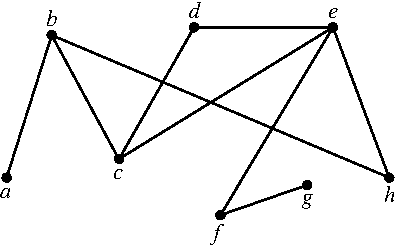
\includegraphics[height=1.75in]{distance-graph}
\caption{A graph with 3 simple cycles.}
\label{dg}
\end{figure}

As in digraphs, the length of a path is the total number of times it traverses edges,
which is \emph{one less} than its length as a sequence of vertices.  For example, the
length~6 path A,B,C,D,E,F,G is actually a sequence of seven vertices.

A \emph{\idx{cycle}} can be described by a path \iffalse of length two or
more\fi that begins and ends with the same vertex.  For example,
B,C,D,E,C,B is a cycle in the graph in Figure~\ref{dg}.  This path
suggests that the cycle begins and ends at vertex B, but a cycle isn't
intended to have a beginning and end, and can be described by \emph{any}
of the paths that go around it.  For example, D,E,C,B,C,D describes this
same cycle as though it started and ended at D, and D,C,B,C,E,D describes
the same cycle as though it started and ended at D but went in the
opposite direction.  (By convention, a single vertex is a length 0 cycle
beginning and ending at the vertex.)

All the paths that describe the same cycle have the same length which is defined to
be the \term{length of the cycle}.  (Note that this implies that going around the
same cycle twice is considered to be different than going around it once.)

A \index{simple cycle}\emph{simple} cycle is a cycle that doesn't cross or
backtrack on itself.  For example, the graph in Figure~\ref{dg} has three
simple cycles B,H,E,C,B and C,D,E,C and B,C,D,E,H,B.  More precisely, a
simple cycle is a cycle that can be described by a path of length at least
three whose vertices are all different except for the beginning and end
vertices.  So in contrast to simple \emph{paths}, the length of a simple
\emph{cycle} is the \emph{same} as the number of distinct vertices that
appear in it.

From now on we'll stop being picky about distinguishing a cycle from a
path that describes it, and we'll just refer to the path as a cycle.
\footnote{Technically speaking, we haven't ever defined what a cycle
\emph{is}, only how to describe it with paths.  But we won't need an
abstract definition of cycle, since all that matters about a cycle is which
paths describe it.}

Simple cycles are especially important, so we will give a proper
definition of them.  Namely, we'll define a simple cycle in $G$ to be a
\emph{subgraph} of $G$ that looks like a cycle that doesn't cross itself.
Formally:
\begin{definition}
A \term{subgraph}, $G'$, of a graph, $G$, is a graph whose vertices, $V'$,
are a subset of the vertices of $G$ and whose edges are a subset
of the edges of $G$.
\end{definition}
Notice that since a subgraph is itself a graph, the endpoints of every
edge of $G'$ must be vertices in $V'$.
\begin{definition}
  For $n \ge 3$, let \term{$C_n$} be the graph with vertices $1,\dots, n$
  and edges
\[
\edge{1}{2},\ \ \edge{2}{3},\ \ \dots,\ \ \edge{(n-1)}{n},\ \ \edge{n}{1}.
\]

A graph is a \term{simple cycle} of length $n$ iff it is isomorphic to $C_n$
for some $n \ge 3$.  A \term{simple cycle of a graph}, $G$, is a subgraph
of $G$ that is a simple cycle.
\end{definition}
This definition formally captures the idea that simple cycles don't
have direction or beginnings or ends.


\subsection{Connected Components}
\begin{definition}
  Two vertices in a graph are said to be \term{connected} when there is a
  path that begins at one and ends at the other.  By convention, every
  vertex is considered to be connected to itself by a path of length zero.
\end{definition}

\begin{editingnotes}

Now if there is a path from vertex $u$ to vertex $v$, then $v$ is
connected to $u$ by the reverse path, so connectedness is a symmetric
relation.  Also, if there is a path from $u$ to $v$, and also a path from
$v$ to $w$, then these two paths can be combined to form a path from $u$
to $w$.  So the connectedness relation is transitive.  It is also
reflexive, since every vertex is by definition connected to itself by a
path of length zero.

\end{editingnotes}

The diagram in Figure~\ref{fig:3comp} looks like a picture of three
graphs, but is intended to be a picture of \emph{one} graph.  This graph
consists of three pieces (subgraphs).  Each piece by itself is connected,
but there are no paths between vertices in different pieces.

\begin{editingnotes}

\begin{figure}[htbp]
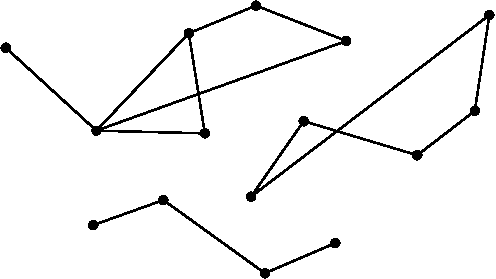
\includegraphics[height=1.5in]{3comp}
\caption{One graph with 3 connected components.}
\label{fig:3comp}
\end{figure}

\end{editingnotes}

\begin{figure}[htbp]
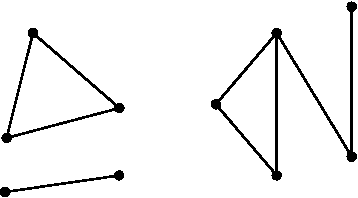
\includegraphics[height=1.5in]{connectivity-graphs}
\caption{One graph with 3 connected components.}
\label{fig:3comp}
\end{figure}

\begin{definition}\label{def:connected-graph}
A graph is said to be \term{connected} when every pair of vertices are
connected.
\end{definition}
These connected pieces of a graph are called its \term{connected
components}.  A rigorous definition is easy: a connected component is the
set of all the vertices connected to some single vertex.  So a graph is
connected iff it has exactly one connected component.  The empty graph on
$n$ vertices has $n$ connected components.

\subsection{How Well Connected?}
If we think of a graph as modelling cables in a telephone network, or
oil pipelines, or electrical power lines, then we not only want
connectivity, but we want connectivity that survives component
failure.  A graph is called \emph{$k$-edge connected} if it takes at
least $k$ ``edge-failures'' to disconnect it.  More precisely:

\begin{definition}
  Two vertices in a graph are $k$-\term{edge connected} if they remain
  connected in every subgraph obtained by deleting $k-1$ edges.  A graph
  with at least two vertices is $k$-edge connected\footnote{The
    corresponding definition of connectedness based on deleting vertices
    rather than edges is common in Graph Theory texts and is usually
    simply called ``$k$-connected'' rather than ``$k$-vertex connected.''}
  if every two of its vertices are $k$-edge connected.
\end{definition}

So 1-edge connected is the same as connected for both vertices and graphs.
Another way to say that a graph is $k$-edge connected is that every
subgraph obtained from it by deleting at most $k-1$ edges is connected.
For example, in the graph in Figure~\ref{dg}, vertices B and E are 2-edge
connected, G and E are 1-edge connected, and no vertices are 3-edge
connected.  The graph as a whole is only 1-edge connected.  More
generally, any simple cycle is 2-edge connected, and the complete graph,
$K_n$, is $(n-1)$-edge connected.

If two vertices are connected by $k$ edge-disjoint paths (that is, no
two paths traverse the same edge), then they are obviously $k$-edge
connected.  A fundamental fact, whose ingenious proof we omit,
is \idx{Menger}'s theorem which confirms that the converse is also
true: if two vertices are $k$-edge connected, then there are $k$
edge-disjoint paths connecting them.  It even takes some ingenuity to
prove this for the case $k=2$.

\subsection{Connection by Simple Path}

Where there's a path, there's a simple path.  This is sort of obvious, but
it's easy enough to prove rigorously using the \idx{Well Ordering Principle}.

\begin{lemma}\label{simplepath}
If vertex $u$ is connected to vertex $v$ in a graph, then there is a
simple path from $u$ to $v$.
\end{lemma}

\begin{proof}
Since there is a path from $u$ to $v$, there must, by the Well-ordering
Principle, be a minimum length path from $u$ to $v$.  If the minimum
length is zero or one, this minimum length path is itself a simple path
from $u$ to $v$.
Otherwise, there is a minimum length path
\[
v_0, v_1,\dots, v_k
\]
from $u = v_0$ to $v = v_k$ where $k \geq 2$.  We claim this path must be
simple.
To prove the claim, suppose to the contrary that the path is not simple,
that is, some vertex on the path occurs twice.  This means that there are
integers $i,j$ such that $0 \leq i < j \leq k$ with $v_i= v_j$.  Then
deleting the subsequence
\[
v_{i+1}, \dots v_j
\]
yields a strictly shorter path
\[
v_0, v_1,\dots, v_i,v_{j+1},v_{j+2},\dots, v_k
\]
from $u$ to $v$, contradicting the minimality of the given path.
\end{proof}

Actually, we proved something stronger:
\begin{corollary}\label{ss}
For any path of length $k$ in a graph, there is a simple path of length
\emph{at most} $k$ with the same endpoints.
\end{corollary}

\subsection{The Minimum Number of Edges in a Connected Graph}
The following theorem says that a graph with few edges must have many
connected components.
\begin{theorem} \label{th:connectivity}
Every graph with $v$ vertices and $e$ edges has at least $v - e$ connected
components.
\end{theorem}
Of course for Theorem~\ref{th:connectivity} to be of any use, there must
be fewer edges than vertices.

\begin{proof}
We use induction on the number of edges, $e$.  Let $P(e)$ be the
proposition that
\begin{quote}
for every $v$, every graph with $v$ vertices and $e$ edges has at least
$v-e$ connected components.
\end{quote}

\textbf{Base case:}($e=0$).  In a graph with 0 edges and $v$ vertices,
each vertex is itself a connected component, and so there are exactly $v =
v - 0$ connected components.  So $P(e)$ holds.

\textbf{Inductive step:} Now we assume that the induction hypothesis holds
for every $e$-edge graph in order to prove that it holds for every
$(e+1)$-edge graph, where $e \geq 0$.
Consider a graph, $G$, with $e + 1$ edges and $k$ vertices.  We want to
prove that $G$ has at least $v - (e+1)$ connected components.
To do this, remove an arbitrary edge $\edge{a}{b}$ and call the resulting
graph $G'$.  By the induction assumption, $G'$ has at least $v - e$
connected components.
Now add back the edge $\edge{a}{b}$ to obtain the original graph $G$.  If
$a$ and $b$ were in the same connected component of $G'$, then $G$ has the
same connected components as $G'$, so $G$ has at least $v -e > v - (e+1)$
components.  Otherwise, if $a$ and $b$ were in different connected
components of $G'$, then these two components are merged into one in $G$,
but all other components remain unchanged, reducing the number of
components by 1.  Therefore, $G$ has at least $(v - e) - 1 = v - (e+1)$
connected components.  So in either case, $P(e+1)$ holds.  This completes
the Inductive step.
The theorem now follows by induction.
\end{proof}

\begin{corollary}
\label{cor:n-1}
Every connected graph with $v$ vertices has at least $v - 1$ edges.
\end{corollary}

A couple of points about the proof of Theorem~\ref{th:connectivity} are
worth noticing.  First, we used induction on the number of
edges in the graph.  This is very common in proofs involving graphs, and
so is induction on the number of vertices.  When you're presented with a
graph problem, these two approaches should be among the first you
consider.  The second point is more subtle.  Notice that in the inductive
step, we took an arbitrary $(n+1)$-edge graph, threw out an edge so that
we could apply the induction assumption, and then put the edge back.
You'll see this shrink-down, grow-back process very often in the inductive
steps of proofs related to graphs.  This might seem like needless effort;
why not start with an $n$-edge graph and add one more to get an
$(n+1)$-edge graph?  That would work fine in this case, but opens the door
to a nasty logical error called \term{buildup error}, illustrated in
Problems~\ref{PS_graph_two_ends} and~\ref{CP_pos_deg_but_not_connected}.
Always use shrink-down, grow-back arguments, and you'll never fall into
this trap.
%S08, cp6m, S06 cp5f

%S06 cp5f

%% Connectedness Problems %%%%%%%%%%%%%%%%%%%%%%%%%%%%%%%%%%%%%%%%%%%%%%%%%%%%
\begin{problems}
\classproblems
\pinput{CP_n_dim_hypercube}
\pinput{CP_graph_maximal_connected}
\pinput{CP_Kn_is_very_connected}
\pinput{CP_pos_deg_but_not_connected}
\homeworkproblems
\pinput{PS_Euler_circuits}

% S09.cp6m.2
% S09.cp6t.1

\homeworkproblems
\pinput{PS_tangled_and_mangled_graphs}
\pinput{PS_circuit_graph_with_crossbars}
\end{problems}

%% Trees %%%%%%%%%%%%%%%%%%%%%%%%%%%%%%%%%%%%%%%%%%%%%%%%%%%%%%%%%%%%%%%%%%%%%%
%Used to come after Coloring: proof read for switched references

\section{Trees}\label{trees-sec}
Trees are a fundamental data structure in computer science, and there are
many kinds, such as rooted, ordered, and binary trees.  In this section
we focus on the purest kind of tree.  Namely, we use the term \term{tree} to
mean a connected graph without simple cycles.

A graph with no simple cycles is called \term{acyclic}; so trees are
acyclic connected graphs.

\subsection{Tree Properties}

Here is an example of a tree:

\mfigure{!}{1.5in}{tree-example}

A vertex of degree at most one is called a \term{leaf}.  In this example, there are 5~leaves. Note
that the only case where a tree can have a vertex of degree zero is a graph with a single
vertex.

The graph shown above would no longer be a tree if any edge were removed,
because it would no longer be connected.  The graph would also not remain
a tree if any edge were added between two of its vertices, because then it
would contain a simple cycle.  Furthermore, note that there is a unique
path between every pair of vertices.  These features of the example tree
are actually common to all trees.

\begin{theorem}\label{th:treeprops}
Every tree has the following properties:

\begin{enumerate}
\item Any connected subgraph is a tree.\label{asub}

\item There is a unique simple path between every pair of vertices.
\item Adding an edge between two vertices creates a cycle.
\item Removing any edge disconnects the graph.
\item If it has at least two vertices, then it has at least two leaves.
\item The number of vertices is one larger than the number of edges.
\end{enumerate}
\end{theorem}

\begin{proof}
\begin{enumerate}

\item A simple cycle in a subgraph is also a simple cycle in
the whole graph, so any subgraph of an acyclic graph must also be acyclic.
If the subgraph is also connected, then by definition, it is a tree.

\item There is at least one path, and hence one simple path, between every
pair of vertices, because the graph is connected.  Suppose that there are
two different simple paths between vertices $u$ and $v$.  Beginning at
$u$, let $x$ be the first vertex where the paths diverge, and let $y$ be
the next vertex they share.  Then there are two simple paths from $x$ to
$y$ with no common edges, which defines a simple cycle.  This is a
contradiction, since trees are acyclic.  Therefore, there is exactly one
simple path between every pair of vertices.

\mfigure{!}{1in}{unique-path}

\item An additional edge $\edge{u}{v}$ together with the unique path
between $u$ and $v$ forms a simple cycle.

\item Suppose that we remove edge $\edge{u}{v}$.  Since the tree
contained a unique path between $u$ and $v$, that path must have been
$\edge{u}{v}$.  Therefore, when that edge is removed, no path remains,
and so the graph is not connected.

\item Let $v_1, \dots, v_m$ be the sequence of vertices on a longest
simple path in the tree.  Then $m \geq 2$, since a tree with two vertices
must contain at least one edge.  There cannot be an edge $\edge{v_1}{v_i}$
for $2 < i \leq m$; otherwise, vertices $v_1, \dots, v_i$ would from a
simple cycle.  Furthermore, there cannot be an edge $\edge{u}{v_1}$ where
$u$ is not on the path; otherwise, we could make the path longer.
Therefore, the only edge incident to $v_1$ is $\edge{v_1}{v_2}$, which
means that $v_1$ is a leaf.  By a symmetric argument, $v_m$ is a second
leaf.

\item We use induction on the number of vertices.  For a tree with a
single vertex, the claim holds since it has no edges and $0 + 1 = 1$ vertex.
Now suppose that the claim holds for all $n$-vertex trees and consider an
$(n+1)$-vertex tree, $T$.  Let $v$ be a leaf of the tree.
You can verify that deleting a vertex of degree 1 (and its incident edge)
from any connected graph leaves a connected subgraph.  So by~\ref{asub}.,
deleting $v$ and its incident edge gives a smaller tree, and this smaller
tree has one more vertex than edge by induction.  If we re-attach the
vertex, $v$, and its incident edge, then the equation still holds because
the number of vertices and number of edges both increase by 1.  Thus, the
claim holds for $T$ and, by induction, for all trees.
\end{enumerate}
\end{proof}
Various subsets of these properties provide alternative characterizations
of trees, though we won't prove this.  For example, a \emph{connected}
graph with a number of vertices one larger than the number of edges is
necessarily a tree.  Also, a graph with unique paths between every pair of
vertices is necessarily a tree.

\subsection{Spanning Trees}
Trees are everywhere.  In fact, every connected graph contains a
subgraph that is a tree with the same vertices as the graph.  This is a
called a \term{spanning tree} for the graph.  For example, here is a
connected graph with a spanning tree highlighted.
\mfigure{!}{1.5in}{spanning-tree}

\begin{theorem}
Every connected graph contains a spanning tree.
\end{theorem}

\begin{proof}
Let $T$ be a connected subgraph of $G$, with the same vertices as $G$, and
with the smallest number of edges possible for such a subgraph.  We show
that $T$ is acyclic by contradiction.  So suppose that $T$ has a cycle
with the following edges:
\[
\edge{v_0}{v_1}, \edge{v_1}{v_2}, \dots, \edge{v_n}{v_0}
\]
Suppose that we remove the last edge, $\edge{v_n}{v_0}$.  If a pair of
vertices $x$ and $y$ was joined by a path not containing
$\edge{v_n}{v_0}$, then they remain joined by that path.  On the other
hand, if $x$ and $y$ were joined by a path containing $\edge{v_n}{v_0}$,
then they remain joined by a path containing the remainder of the cycle.
So all the vertices of $G$ are still connected after we remove an edge
from $T$.  This is a contradiction, since $T$ was defined to be a minimum
size connected subgraph with all the vertices of $G$.  So $T$ must be
acyclic.
\end{proof}

\begin{editingnotes}

\subsection{Tree Variations}
Trees come up often in computer science.  For example, information is
often stored in tree-like data structures and the execution of many
recursive programs can be regarded as a traversal of a tree.
There are many varieties of trees.  For example, a \term{rooted tree}
is a tree with one vertex identified as the \term{root}.  Let
$\edge{u}{v}$ be an edge in a rooted tree such that $u$ is closer to
the root than $v$.  Then $u$ is the \term{parent} of $v$, and $v$ is
a \term{child} of $u$.
\mfigure{!}{1.5in}{rooted-tree}
In the tree above, suppose that we regard vertex $A$ as the
root.  Then $E$ and $F$ are the children of $B$, and $A$ is the parent
of $B$, $C$, and $D$.
A \term{binary} tree is a rooted tree in which every vertex has at most
two children.  Here is an example, where the topmost vertex is the
root.
\mfigure{!}{1.5in}{binary-tree}
In an \term{ordered, binary} tree, the children of a vertex $v$ are
distinguished.  One is called the \term{left child} of $v$, and the
other is called the \term{right child}.  For example, if we regard the
two binary trees below as unordered, then they are equivalent.
However, if we regard these trees as ordered, then they are different.
\mfigure{!}{1.5in}{ordered-trees}

\end{editingnotes}

\begin{editingnotes}

Problem~\ref{PS_Euler_circuits} presents most of this as a homework
problem.

\section{Traversing a Graph}
Can you walk every hallway in the Museum of Fine Arts \emph{exactly
once}?  If we represent hallways and intersections with edges and
vertices, then this reduces to a question about graphs.  For example,
could you visit every hallway exactly once in a museum with this
floorplan?

\mfigure{!}{1.5in}{euler-tour}

\subsection{Euler Tours and Hamiltonian Cycles}

The entire field of graph theory began when Euler asked whether the seven
bridges of K\"onigsberg could all be traversed exactly once--- essentially
the same question we asked about the Museum of Fine Arts.  In his honor,
an \term{Euler walk} is a defined to be a path that traverses every edge
in a graph exactly once.  Similarly, an \term{Euler tour} is an Euler walk
that starts and finishes at the same vertex, that is a cycle that
traverses every edge exactly once.  Graphs with Euler tours and Euler
walks both have simple characterizations.
\begin{theorem}
A graph has an Euler tour iff it is connected and every vertex has even
degree.
\end{theorem}
\begin{proof}
Suppose a graph has an Euler tour.  Every pair of vertices must appear in
the tour, so the graph is connected.  Moreover, a vertex that appears $k$
times in the tour must have degree $2k$, so every vertex of the graph has
even degree.

\textcolor{red}{Unconvincing!}

Conversely, suppose every vertex in a graph, $G$, has even degree.  Let $W
= (v_0,\dots,v_n)$ be the longest path in $G$ that traverses every edge
\emph{at most} once.  Now $W$ must traverse every edge incident to
$v_n$; otherwise, the path could be extended.  In particular, the $W$
traverses two of these edges each time it passes through $v_n$, and it
traverses $\edge{v_{n-1}}{v_n}$ at the end.  This accounts for an odd
number of edges, but the degree of $v_n$ is even by assumption.
Therefore, the $W$ must also begin at $v_n$; that is, $v_0 = v_n$.
Suppose that $W$ is not an Euler tour.  Because $G$ is a connected
graph, we can find an edge not in $W$ but incident to some vertex in
$W$.  Call this edge $\edge{u}{v_i}$.  But then we can construct a
longer walk:
%
\[
u, \edge{u}{v_i}, v_i, \edge{v_i}{v_{i+1}},
\dots,
\edge{v_{n-1}}{v_n}, v_n, \edge{v_0}{v_1},
\dots,
\edge{v_{i-1}}{v_i}, v_i
\]
%
This contradicts the definition of $W$, so $W$ must be an
Euler tour after all.
\end{proof}

\begin{corollary}
A connected graph has an Euler walk if and only if either 0 or 2
vertices have odd degree.
\end{corollary}

Hamiltonian cycles are the unruly cousins of Euler tours.  A
\term{Hamiltonian cycle} is walk that starts and ends at the same vertex
and visits every \emph{vertex} in a graph exactly once.  There is no
simple characterization of all graphs with a Hamiltonian cycle.  In
fact, determining whether a given graph has a Hamiltonian cycle is is
the same category of problem as the SAT problem of
Section~\ref{SAT_sec}: you get a million dollars for finding an
efficient way to determine when a graph has a Hamiltonian cycle ---or
for proving that no procedure works efficiently on all graphs.

\end{editingnotes}

%% Trees Problems %%%%%%%%%%%%%%%%%%%%%%%%%%%%%%%%%%%%%%%%%%%%%%%%%%%%%%%%%%%%%
\begin{problems}
\classproblems
\pinput{CP_graph_edge_mark}
\pinput{CP_spanning_tree_proc}
\pinput{CP_tree_characterizations}
%\pinput{CP_23_high_priority_servers}

\homeworkproblems
\pinput{PS_average_degree_of_tree_and_simple_path}
% S09.cp6t.2
% S09.cp6t.3
\end{problems}

%% Coloring Graphs %%%%%%%%%%%%%%%%%%%%%%%%%%%%%%%%%%%%%%%%%%%%%%%%%%%%%%%%%%%%
%Used to come before Trees: proof read for switched references

\hyperdef{graph}{coloring}{\section{Coloring Graphs}}

In section~\ref{sexam},
we used edges to indicate an affinity between two nodes, but having an
edge represent a \emph{conflict} between two nodes also turns out to be
really useful.

\section{Modelling Scheduling Conflicts}

Each term the MIT Schedules Office must assign a time slot for each final
exam.  This is not easy, because some students are taking several classes
with finals, and a student can take only one test during a particular time
slot.  The Schedules Office wants to avoid all conflicts.  Of course, you
can make such a schedule by having every exam in a different slot, but
then you would need hundreds of slots for the hundreds of courses, and
exam period would run all year!  So, the Schedules Office would also like
to keep exam period short.  The Schedules Office's problem is easy to
describe as a graph.  There will be a vertex for each course with a final
exam, and two vertices will be adjacent exactly when some student is
taking both courses.  For example, suppose we need to schedule exams for
6.041, 6.042, 6.002, 6.003 and 6.170.  The scheduling graph might look
like this:

\mfigure{!}{1.5in}{finals-subject-labels}

6.002 and 6.042 cannot have an exam at the same time since there are
students in both courses, so there is an edge between their nodes.  On the
other hand, 6.042 and 6.170 can have an exam at the same time if they're
taught at the same time (which they sometimes are), since no student can
be enrolled in both (that is, no student \emph{should} be enrolled in both
when they have a timing conflict).  Next, identify each time slot with a
color.  For example, Monday morning is red, Monday afternoon is blue,
Tuesday morning is green, etc.

Assigning an exam to a time slot is now equivalent to coloring the
corresponding vertex.  The main constraint is that \emph{adjacent vertices
  must get different colors} ---otherwise, some student has two exams at
the same time.  Furthermore, in order to keep the exam period short, we
should try to color all the vertices using as \emph{few different colors
  as possible}.  For our example graph, three colors suffice:

\mfigure{!}{1.5in}{finals-colored}

This coloring corresponds to giving one final on Monday morning (red),
two Monday afternoon (blue), and two Tuesday morning (green).
Can we use fewer than three colors?  No! We can't use only two colors
since there is a triangle in the graph, and three vertices in a triangle
must all have different colors.

This is an example of what is a called a \term{graph coloring problem}:
given a graph $G$, assign colors to each node such that adjacent nodes
have different colors.  A color assignment with this property is called a
\term{valid coloring} of the graph ---a ``\term{coloring},'' for short.  A
graph $G$ is $k$-\term{colorable} if it has a coloring that uses at most
$k$ colors.
\begin{definition}
  The minimum value of $k$ for which a graph, $G$, has a valid coloring is
  called its \term{chromatic number}, $\chi(G)$.
\end{definition}

In general, trying to figure out if you can color a graph with a fixed
number of colors can take a long time.  It's a classic example of a
problem for which no fast algorithms are known.  In fact, it is easy to
check if a coloring works, but it seems really hard to find it (if you
figure out how, then you can get a \$1 million Clay prize).


\subsection{Degree-bounded Coloring}
There are some simple graph properties that give useful upper bounds on
colorings.  For example, if we have a bound on the degrees of all the
vertices in a graph, then we can easily find a coloring with only one more
color than the degree bound.

\begin{theorem}\label{k+1-colorable}
A graph with maximum degree at most $k$ is $(k+1)$-colorable.
\end{theorem}

Unfortunately, if you try induction on $k$, it will lead to disaster.  It
is not that it is impossible, just that it is extremely painful and would
ruin you if you tried it on an exam.  Another option, especially with
graphs, is to change what you are inducting on.  In graphs, some good
choices are $n$, the number of nodes, or $e$, the number of edges.

\begin{proof}
We use induction on the number of vertices in the graph, which we
denote by $n$.  Let $P(n)$ be the proposition that an $n$-vertex graph
with maximum degree at most $k$ is $(k+1)$-colorable.

\textbf{Base case}: ($n=1$) A 1-vertex graph has maximum degree 0 and is
1-colorable, so $P(1)$ is true.

\textbf{Inductive step}: Now assume that $P(n)$ is true, and let $G$ be an
$(n+1)$-vertex graph with maximum degree at most $k$.  Remove a vertex $v$
(and all edges incident to it), leaving an $n$-vertex subgraph, $H$.  The
maximum degree of $H$ is at most $k$, and so $H$ is $(k+1)$-colorable by
our assumption $P(n)$.  Now add back vertex $v$.  We can assign $v$ a
color different from all its adjacent vertices, since there are at
most $k$ adjacent vertices and $k+1$ colors are available.  Therefore, $G$
is $(k+1)$-colorable.  This completes the inductive step, and the theorem
follows by induction.
\end{proof}

Sometimes $k+1$ colors is the best you can do.  For example, in the
complete graph, $K_n$, every one of its $n$ vertices is adjacent to all
the others, so all $n$ must be assigned different colors.  Of course $n$
colors is also enough, so $\chi(K_n)=n$.  So $K_{k+1}$ is an example where
Theorem~\ref{k+1-colorable} gives the best possible bound.  This means
that Theorem~\ref{k+1-colorable} also gives the best possible bound for
\emph{any} graph with degree bounded by $k$ that has $K_{k+1}$ as a
subgraph.
\begin{editingnotes}

The complete graph, $K_n$, is also called a size $n$ \term{clique},
just like a clique of friends, where nodes represent the people and an
edge represents the friendship relationship.\footnote{ When speaking
of friends, clique is usually pronounced similar to click.  However,
for some reason, graph theorists think that the word clique rhymes
with geek.}
%\mfigure{!}{1.5in}{complete-graph}
\end{editingnotes}

But sometimes $k+1$ colors is far from the best that you can do.  Here's
an example of an $n$-node star graph for $n=7$:
\mfigure{!}{1.5in}{star-graph}
In the $n$-node star graph, the maximum degree is $n-1$, but the star only
needs $2$ colors!

\subsection{Why coloring?}

One reason coloring problems come all the time is because scheduling
conflicts are so common.  For example, at Akamai, a new version of
software is deployed over each of 20,000 servers every few days.  The
updates cannot be done at the same time since the servers need to be taken
down in order to deploy the software.  Also, the servers cannot be handled
one at a time, since it would take forever to update them all (each one
takes about an hour).  Moreover, certain pairs of servers cannot be taken
down at the same time since they have common critical functions.  This
problem was eventually solved by making a 20,000 node conflict graph and
coloring it with 8 colors -- so only 8 waves of install are needed!
Another example comes from the need to assign frequencies to radio
stations.  If two stations have an overlap in their broadcast area, they
can't be given the same frequency.  Frequencies are precious and
expensive, so you want to minimize the number handed out.  This amounts to
finding the minimum coloring for a graph whose vertices are the stations
and whose edges are between stations with overlapping areas.

Coloring also comes up in allocating registers for program variables.
While a variable is in use, its value needs to be saved in a register, but
registers can often be reused for different variables.  But two variables
need different registers if they are referenced during overlapping
intervals of program execution.  So register allocation is the coloring
problem for a graph whose vertices are the variables; vertices are
adjacent if their intervals overlap, and the colors are registers.

Finally, there's the famous map coloring problem stated in
Propostion~\ref{4colorprop}.  The question is how many colors are
needed to color a map so that adjacent territories get different
colors?  This is the same as the number of colors needed to color a
graph that can be drawn in the plane without edges crossing.  A proof
that four colors are enough for the \emph{planar} graphs was acclaimed
when it was discovered about thirty years ago.  Implicit in that proof
was a 4-coloring procedure that takes time proportional to the number
of vertices in the graph (countries in the map).  On the other hand,
it's another of those million dollar prize questions to find an
efficient procedure to tell if a planar graph really \emph{needs} four
colors or if three will actually do the job.  But it's always easy to
tell if an \emph{arbitrary} graph is 2-colorable, as we show in
section~\ref{bipartitesec}.  Finally, in
section~\ref{planar_graphs_sec}, we'll develop enough planar graph
theory to present an easy proof at least that planar graphs are
5-colorable.

%% Coloring Graphs Problems %%%%%%%%%%%%%%%%%%%%%%%%%%%%%%%%%%%%%%%%%%%%%%%%%%%
\begin{problems}
\classproblems
\pinput{CP_chromatic_number}

% S09.cp6r.1
% S09.cp6r.2

\homeworkproblems
\pinput{PS_TA_recitation_graph_coloring}
\pinput{PS_graph_colorable}
%\pinput{PS_simple_triangle_free_graph_coloring}

\examproblems
\pinput{FP_coloring_false_proof}

\end{problems}

%% Bipartite Matchings %%%%%%%%%%%%%%%%%%%%%%%%%%%%%%%%%%%%%%%%%%%%%%%%%%%%%%%%
\hyperdef{bipartite}{matching}{\section{Bipartite Matchings}}\label{bipartitesec}

\subsection{Bipartite Graphs}\label{bipartitesubsec}
There were two kinds of vertices in the ``Sex in America'' graph ---males
and females, and edges only went between the two kinds.  Graphs like this
come up so frequently they have earned a special name ---they are called
\emph{bipartite graphs}.

\begin{definition}
A \term{bipartite graph} is a graph together with a partition of its
vertices into two sets, $L$ and $R$, such that every edge is incident to a
vertex in $L$ and to a vertex in $R$.
\end{definition}

So every bipartite graph looks something like this:

\mfigure{!}{2in}{bipartite}

Now we can immediately see how to color a bipartite graph using only two
colors: let all the $L$ vertices be black and all the $R$ vertices be
white.  Conversely, if a graph is 2-colorable, then it is bipartite with
$L$ being the vertices of one color and $R$ the vertices of the other
color.  In other words,
\begin{quote}
``bipartite'' is a synonym for ``\term{2-colorable}.''
\end{quote}
The following Lemma gives another useful characterization of bipartite
graphs.

\hyperdef{odd}{cycle}
{\begin{theorem}\label{odd-cycle}
A graph is bipartite iff it has no odd-length cycle.
\end{theorem}}
The proof of Theorem~\ref{odd-cycle} is left to
Problem~\ref{PS_no_odd_length_cycles}.

\subsection{Bipartite Matchings}

The \term{bipartite matching} problem resembles the stable Marriage
Problem in that it concerns a set of girls and a set of at least as many
boys.  There are no preference lists, but each girl does have some boys
she likes and others she does not like.  In the bipartite matching
problem, we ask whether every girl can be paired up with a boy that she
likes.  Any particular matching problem can be specified by a
\idx{bipartite graph} with a vertex for each girl, a vertex for each boy,
and an edge between a boy and a girl iff the girl likes the boy.  For
example, we might obtain the following graph:

\mfigure{!}{2in}{hall-graph}

Now a \term{matching} will mean a way of assigning every girl to a boy so
that different girls are assigned to different boys, and a girl is always
assigned to a boy she likes.  For example, here is one possible matching
for the girls:

\mfigure{!}{2in}{hall-graph-matched}

\idx{Hall's Matching Theorem} states necessary and sufficient conditions
for the existence of a matching in a bipartite graph.  It turns out to be
a remarkably useful mathematical tool.

\begin{solution}
, a hammer that bashes
many problems.  Moreover, it is the tip of a conceptual iceberg, a special
case of the ``max-flow, min-cut theorem'' which is in turn a byproduct of
``linear programming duality,'' one of the central ideas of algorithmic
theory.
\end{solution}

\subsection{The Matching Condition}

We'll state and prove Hall's Theorem using girl-likes-boy terminology.
Define \emph{the set of boys liked by a given set of girls} to consist of
all boys liked by at least one of those girls.  For example, the set of
boys liked by Martha and Jane consists of Tom, Michael, and Mergatroid.
For us to have any chance at all of matching up the girls, the following
\term{matching condition} must hold:

\bigskip
\begin{center}
\emph{Every subset of girls likes at least as large a set of boys.}
\end{center}
\bigskip

For example, we can not find a matching if some 4~girls like only 3~boys.
Hall's Theorem says that this necessary condition is actually sufficient;
if the matching condition holds, then a matching exists.

\begin{theorem}
A matching for a set of girls $G$ with a set of boys $B$ can be found if
and only if the matching condition holds.
\end{theorem}

\begin{proof}
First, let's suppose that a matching exists and show that the matching condition
holds.  Consider an arbitrary subset of girls.  Each girl likes at least the boy she
is matched with.  Therefore, every subset of girls likes at least as large a set of
boys.  Thus, the matching condition holds.

Next, let's suppose that the matching condition holds and show that a matching
exists.  We use strong induction on $\card{G}$, the number of girls.

\textbf{Base Case}: ($\card{G}=1$) If $\card{G} = 1$, then the
matching condition implies that the lone girl likes at least one boy, and so a
matching exists.

\textbf{Inductive Step}: Now suppose that $\card{G} \geq 2$.  There are two cases:

\begin{itemize}

\item[Case 1:] Every proper subset of girls likes a \emph{strictly larger} set of
  boys.  In this case, we have some latitude: we pair an arbitrary girl with a boy
  she likes and send them both away.  The matching condition still holds for the
  remaining boys and girls, so we can match the rest of the girls by induction.

\item[Case 2:] Some proper subset of girls $X \subset G$ likes an \emph{equal-size}
  set of boys $Y \subset B$.  We match the girls in $X$ with the boys in $Y$ by
  induction and send them all away.  We can also match the rest of the girls by
  induction if we show that the matching condition holds for the remaining boys and
  girls.  To check the matching condition for the remaining people, consider an
  arbitrary subset of the remaining girls $X' \subseteq (G - X)$, and let $Y'$ be the
  set of remaining boys that they like.  We must show that
  $\card{X'} \leq \card{Y'}$.  Originally, the combined set of girls $X \cup X'$
  liked the set of boys $Y \cup Y'$.  So, by the matching condition, we know:
%
\[
\card{X \cup X'}  \leq  \card{Y \cup Y'}
\]
%
We sent away $\card{X}$ girls from the set on the left (leaving $X'$) and sent away
an equal number of boys from the set on the right (leaving $Y'$).  Therefore, it must
be that $\card{X'}
\leq \card{Y'}$ as claimed.
\end{itemize}

So there is in any case a matching for the girls, which completes the proof of the
Inductive step.   The theorem follows by induction.
\end{proof}

The proof of this theorem gives an algorithm for finding a matching in a bipartite
graph, albeit not a very efficient one.  However, efficient algorithms for finding a
matching in a bipartite graph do exist.  Thus, if a problem can be reduced to finding
a matching, the problem is essentially solved from a computational perspective.

\subsection{A Formal Statement}

Let's restate \idx{Hall's Theorem} in abstract terms so that you'll not always be
condemned to saying, ``Now this group of little girls likes at least as many little
boys...''
% A \emph{matching} in a graph is an injection on the set of vertices
% that only maps a vertex to an adjacent vertex.  Albert: Do you mean
% in the bipartite case?  Otherwise, wouldn't the injection
% f(i)->i+1(mod n) on {1,..,n} determine the cycle C_n and an
% injection?

% Also, is it true that, in this class, an injection/function on $L$
% need only have a domain that is a subset of $L$?  If not I'll need
% to modify the next paragraph.
%

% % CLIFF: Thanks for your correction.  My def with injections (which indeed
% % may be partial) was a failed attempt to be slick.  But given that it's
% % wrong, there's no point in hanging onto injections, so I've revised as
% % follows:

A \term{matching} in a graph, $G$, is a set of edges such that no two edges in the
set share a vertex.  A matching is said to \emph{cover} a set, $L$, of vertices iff
each vertex in $L$ has an edge of the matching incident to it.  In any graph, the set
$N(S)$, of \term{neighbors}\footnote{An equivalent definition of $N(S)$ uses
relational notation: $N(S)$ is simply the image, $SR$, of $S$ under the adjacency
relation, $R$, on vertices of the graph.} of some set, $S$, of vertices is the set of
all vertices adjacent to some vertex in $S$.  That is,
\[
N(S) \eqdef \set{r \suchthat \edge{s}{r}\text{ is an edge for some }s \in S}.
\]
$S$ is called a \term{bottleneck} if
\[
\card{S} > \card{N(S)}.
\]

\begin{theorem}[\idx{Hall's Theorem}]
  Let $G$ be a bipartite graph with vertex partition $L,R$.  There is matching in $G$
  that covers $L$ iff no subset of $L$ is a bottleneck.
\end{theorem}

\subsubsection{An Easy Matching Condition}
The bipartite matching condition requires that \emph{every} subset of girls has a
certain property.  In general, verifying that every subset has some property, even if
it's easy to check any particular subset for the property, quickly becomes
overwhelming because the number of subsets of even relatively small sets is enormous
---over a billion subsets for a set of size 30.  However, there is a simple property
of vertex degrees in a bipartite graph that guarantees a match and is very easy to
check.  Namely, call a bipartite graph \term*{degree-constrained} if vertex degrees
on the left are at least as large as those on the right.  More precisely,
\hyperdef{degree}{constrained}{
\begin{definition}\label{degree-constrained_def}
A bipartite graph $G$ with vertex partition $L,R$ is
\term{degree-constrained} if $\degr{l} \geq \degr{r}$ for every $l \in L$
and $r \in R$.
\end{definition}}
Now we can always find a matching in a degree-constrained bipartite graph.
\begin{lemma}\label{degree-constrained_lemma}
Every degree-constrained bipartite graph satisifies the matching condition.
\end{lemma}

\begin{proof}
Let $S$ be any set of vertices in $L$.  The number of edges incident to vertices in
$S$ is exactly the sum of the degrees of the vertices in $S$.  Each of these edges is
incident to a vertex in $N(S)$ by definition of $N(S)$.  So the sum of the degrees of
the vertices in $N(S)$ is at least as large as the sum for $S$.  But since the degree
of every vertex in $N(S)$ is at most as large as the degree of every vertex in $S$,
there would have to be at least as many terms in the sum for $N(S)$ as in the sum for
$S$.  So there have to be at least as many vertices in $N(S)$ as in $S$, proving that
$S$ is not a bottleneck.  So there are no bottlenecks, proving that the
degree-constrained graph satisifies the matching condition.
\end{proof}
Of course being degree-constrained is a very strong property, and lots of graphs that
aren't degree-constrained have matchings.  But we'll see examples of
degree-constrained graphs come up naturally in some later applications.

%% Bipartite Matchings Problems %%%%%%%%%%%%%%%%%%%%%%%%%%%%%%%%%%%%%%%%%%%%%%%
% S09.cp6r.3
% S09.cp6r.4

\begin{problems}
\classproblems
\pinput{CP_student_clubs}
\pinput{CP_latin_squares}

\examproblems
\pinput{MQ_bipartite-matching_recitations}

\homeworkproblems
\pinput{PS_no_odd_length_cycles}
\pinput{PS_cards_in_4_rows_13_columns}
\pinput{PS_bipartite_matching_virtues}
\end{problems}

\newcommand{\embed}[1]{\mathcal{#1}}  %% may be worth moving to mcs.tex?

%\hyperdef{planar}{graphs}{\chapter{Planar Graphs}\label{planar-graphs-chapter}}

\hyperdef{planar}{graphs}{\section{Planar Graphs}\label{planar_graphs_sec}}

\subsection*{Drawing Graphs in the Plane}

Here are three dogs and three houses.

%\mfigure{!}{1.5in}{dog-houses}
\begin{center}
\setlength{\unitlength}{2000sp}%{3947sp}%
%
\begingroup\makeatletter\ifx\SetFigFont\undefined%
\gdef\SetFigFont#1#2#3#4#5{%
  \reset@font\fontsize{#1}{#2pt}%
  \fontfamily{#3}\fontseries{#4}\fontshape{#5}%
  \selectfont}%
\fi\endgroup%
\begin{picture}(5424,2793)(1039,-3742)
%\thinlines
{\color[rgb]{0,0,0}\put(1201,-1861){\framebox(450,450){}}
}%
{\color[rgb]{0,0,0}\put(1051,-1411){\line( 1, 0){750}}
\put(1801,-1411){\line(-2, 3){300}}
\put(1501,-961){\line(-1,-1){450}}
}%
{\color[rgb]{0,0,0}\put(3451,-1861){\framebox(450,450){}}
}%
{\color[rgb]{0,0,0}\put(3301,-1411){\line( 1, 0){750}}
\put(4051,-1411){\line(-2, 3){300}}
\put(3751,-961){\line(-1,-1){450}}
}%
{\color[rgb]{0,0,0}\put(5851,-1861){\framebox(450,450){}}
}%
{\color[rgb]{0,0,0}\put(5701,-1411){\line( 1, 0){750}}
\put(6451,-1411){\line(-2, 3){300}}
\put(6151,-961){\line(-1,-1){450}}
}%
\put(3451,-3661){\makebox(0,0)[lb]{\smash{{\SetFigFont{17}{20.4}{\rmdefault}{\bfdefault}{\updefault}{\color[rgb]{0,0,0}Dog}%
}}}}
\put(5851,-3661){\makebox(0,0)[lb]{\smash{{\SetFigFont{17}{20.4}{\rmdefault}{\bfdefault}{\updefault}{\color[rgb]{0,0,0}Dog}%
}}}}
\put(1201,-3661){\makebox(0,0)[lb]{\smash{{\SetFigFont{17}{20.4}{\rmdefault}{\bfdefault}{\updefault}{\color[rgb]{0,0,0}Dog}%
}}}}
\end{picture}%

\end{center}

Can you find a path from each dog to each house such that no
two paths intersect?

A \emph{quadapus} is a little-known animal similar to an octopus,
but with four arms.  Here are five quadapi resting on the seafloor:

%%%%%%%%%%%%.fig

%\mfigure{!}{2in}{quadapi}
\begin{center}
\setlength{\unitlength}{2000sp}%{3947sp}%
%
\begingroup\makeatletter\ifx\SetFigFont\undefined%
\gdef\SetFigFont#1#2#3#4#5{%
  \reset@font\fontsize{#1}{#2pt}%
  \fontfamily{#3}\fontseries{#4}\fontshape{#5}%
  \selectfont}%
\fi\endgroup%
\begin{picture}(11049,5049)(589,-5248)
{\color[rgb]{0,0,0}%\thinlines
\put(4688,-1673){\oval(524,524)}
}%
{\color[rgb]{0,0,0}\put(1913,-2948){\oval(524,524)}
}%
{\color[rgb]{0,0,0}\put(4538,-3923){\oval(524,524)}
}%
{\color[rgb]{0,0,0}\put(7838,-3098){\oval(524,524)}
}%
{\color[rgb]{0,0,0}\put(9713,-1748){\oval(524,524)}
}%
{\color[rgb]{0,0,0}\put(4426,-1636){\line(-1, 0){900}}
\multiput(3526,-1636)(-2.67857,-8.03571){57}{\makebox(1.6667,11.6667){\SetFigFont{5}{6}{\rmdefault}{\mddefault}{\updefault}.}}
\put(3376,-2086){\line(-1, 0){750}}
}%
{\color[rgb]{0,0,0}\put(4951,-1711){\line( 5,-3){893.382}}
\put(5851,-2236){\line( 5, 6){442.623}}
\put(6301,-1711){\line( 2,-3){300}}
}%
{\color[rgb]{0,0,0}\multiput(1876,-2686)(1.37838,8.27027){101}{\makebox(1.6667,11.6667){\SetFigFont{5}{6}{\rmdefault}{\mddefault}{\updefault}.}}
\put(2026,-1861){\line( 5, 2){685.345}}
\put(2701,-1561){\line( 0, 1){375}}
}%
{\color[rgb]{0,0,0}\put(2176,-2986){\line( 5, 2){750}}
\put(2926,-2686){\line( 5,-6){510.246}}
\put(3451,-3286){\line( 6, 1){450}}
}%
{\color[rgb]{0,0,0}\put(1951,-3211){\line(-1,-2){300}}
\put(1651,-3811){\line( 5,-6){375}}
\put(2026,-4261){\line( 3, 2){450}}
}%
{\color[rgb]{0,0,0}\put(1651,-2986){\line(-6, 5){612.295}}
\put(1051,-2461){\line(-5,-6){442.623}}
\multiput(601,-2986)(2.02703,-8.10811){75}{\makebox(1.6667,11.6667){\SetFigFont{5}{6}{\rmdefault}{\mddefault}{\updefault}.}}
}%
{\color[rgb]{0,0,0}\multiput(4501,-3661)(1.37838,8.27027){101}{\makebox(1.6667,11.6667){\SetFigFont{5}{6}{\rmdefault}{\mddefault}{\updefault}.}}
\put(4651,-2836){\line( 5, 2){685.345}}
\put(5326,-2536){\line( 0, 1){375}}
}%
{\color[rgb]{0,0,0}\put(4801,-3961){\line( 5, 2){750}}
\put(5551,-3661){\line( 5,-6){510.246}}
\put(6076,-4261){\line( 6, 1){450}}
}%
{\color[rgb]{0,0,0}\put(4576,-4186){\line(-1,-2){300}}
\put(4276,-4786){\line( 5,-6){375}}
\put(4651,-5236){\line( 3, 2){450}}
}%
{\color[rgb]{0,0,0}\put(7576,-3061){\line(-1, 0){900}}
\multiput(6676,-3061)(-2.67857,-8.03571){57}{\makebox(1.6667,11.6667){\SetFigFont{5}{6}{\rmdefault}{\mddefault}{\updefault}.}}
\put(6526,-3511){\line(-1, 0){750}}
}%
{\color[rgb]{0,0,0}\put(7876,-2836){\line(-1, 1){375}}
\put(7501,-2461){\line( 4, 3){600}}
\put(8101,-2011){\line( 0, 1){450}}
}%
{\color[rgb]{0,0,0}\put(8101,-3136){\line( 5,-3){893.382}}
\put(9001,-3661){\line( 5, 6){442.623}}
\put(9451,-3136){\line( 2,-3){300}}
}%
{\color[rgb]{0,0,0}\put(7876,-3361){\line(-2,-5){237.931}}
\put(7651,-3961){\line( 1,-1){600}}
}%
{\color[rgb]{0,0,0}\put(9751,-1486){\line(-1, 1){375}}
\put(9376,-1111){\line( 4, 3){600}}
\put(9976,-661){\line( 0, 1){450}}
}%
{\color[rgb]{0,0,0}\put(9976,-1786){\line( 5,-3){893.382}}
\put(10876,-2311){\line( 5, 6){442.623}}
\put(11326,-1786){\line( 2,-3){300}}
}%
{\color[rgb]{0,0,0}\put(9751,-2011){\line(-2,-5){237.931}}
\put(9526,-2611){\line( 1,-1){600}}
}%
{\color[rgb]{0,0,0}\put(9451,-1711){\line(-5,-1){677.885}}
\put(8776,-1861){\line(-2, 3){692.308}}
\put(8101,-811){\line(-5,-1){1572.115}}
}%
{\color[rgb]{0,0,0}\put(4651,-1936){\line(-1,-4){339.706}}
\put(4276,-3286){\line(-4,-1){1358.823}}
\multiput(2926,-3661)(-1.37838,-8.27027){101}{\makebox(1.6667,11.6667){\SetFigFont{5}{6}{\rmdefault}{\mddefault}{\updefault}.}}
}%
{\color[rgb]{0,0,0}\put(4276,-3886){\line(-3,-2){761.538}}
\multiput(3526,-4411)(2.03287,-8.13149){103}{\makebox(1.6667,11.6667){\SetFigFont{5}{6}{\rmdefault}{\mddefault}{\updefault}.}}
}%
{\color[rgb]{0,0,0}\multiput(4726,-1411)(-1.37387,8.24324){91}{\makebox(1.6667,11.6667){\SetFigFont{5}{6}{\rmdefault}{\mddefault}{\updefault}.}}
\put(4651,-661){\line( 2,-1){1290}}
\put(5926,-1336){\line( 6,-1){1277.027}}
}%
\end{picture}%

\end{center}

Can each quadapus simultaneously shake hands with every other in such a
way that no arms cross?

Informally, a \term{planar graph} is a graph that can be drawn in the
plane so that no edges cross, as in a map of showing the borders of
countries or states.  Thus, these two puzzles are asking whether the
graphs below are planar; that is, whether they can be redrawn so that no
edges cross.  The first graph is called the \term{complete bipartite
  graph}, \idx{$K_{3,3}$}, and the second is \idx{$K_5$}.

%\mfigure{!}{1.5in}{nonplanar}
\begin{center}
\setlength{\unitlength}{3000sp}%{3947sp}%
%
\begingroup\makeatletter\ifx\SetFigFont\undefined%
\gdef\SetFigFont#1#2#3#4#5{%
  \reset@font\fontsize{#1}{#2pt}%
  \fontfamily{#3}\fontseries{#4}\fontshape{#5}%
  \selectfont}%
\fi\endgroup%
\begin{picture}(7366,2266)(2318,-2244)
{\color[rgb]{0,0,0}%\thinlines
\put(2401,-661){\circle{150}}
}%
{\color[rgb]{0,0,0}\put(4726,-661){\circle{150}}
}%
{\color[rgb]{0,0,0}\put(3601,-661){\circle{150}}
}%
{\color[rgb]{0,0,0}\put(3601,-2161){\circle{150}}
}%
{\color[rgb]{0,0,0}\put(2401,-2161){\circle{150}}
}%
{\color[rgb]{0,0,0}\put(4801,-2161){\circle{150}}
}%
{\color[rgb]{0,0,0}\put(8401,-61){\circle{150}}
}%
{\color[rgb]{0,0,0}\put(7201,-961){\circle{150}}
}%
{\color[rgb]{0,0,0}\put(9601,-961){\circle{150}}
}%
{\color[rgb]{0,0,0}\put(7801,-2161){\circle{150}}
}%
{\color[rgb]{0,0,0}\put(9001,-2161){\circle{150}}
}%
{\color[rgb]{0,0,0}\put(2401,-661){\line( 0,-1){1500}}
\put(2401,-2161){\line( 4, 5){1200}}
\put(3601,-661){\line( 4,-5){1200}}
\put(4801,-2161){\line( 0, 1){1500}}
\put(4726,-661){\line(-3,-4){1125}}
\put(3601,-2161){\line(-4, 5){1200}}
}%
{\color[rgb]{0,0,0}\put(3601,-661){\line( 0,-1){1500}}
}%
{\color[rgb]{0,0,0}\put(2401,-661){\line( 5,-3){2426.471}}
}%
{\color[rgb]{0,0,0}\put(4726,-661){\line(-3,-2){2301.923}}
}%
{\color[rgb]{0,0,0}\put(7201,-961){\line( 1,-2){600}}
\put(7801,-2161){\line( 1, 0){1200}}
\put(9001,-2161){\line( 1, 2){600}}
\put(9601,-961){\line(-4, 3){1200}}
\put(8401,-61){\line(-4,-3){1200}}
\put(7201,-961){\line( 1, 0){2400}}
\put(9601,-961){\line(-3,-2){1800}}
\put(7801,-2161){\line( 1, 4){529.412}}
\put(8401,-61){\line( 1,-4){529.412}}
}%
{\color[rgb]{0,0,0}\put(9001,-2161){\line(-3, 2){1800}}
}%
\end{picture}%

\end{center}

In each case, the answer is, ``No--- but almost!''  In fact, each drawing
\emph{would} be possible if any single edge were removed.

Planar graphs have applications in circuit layout and are helpful in
displaying graphical data, for example, program flow charts, organizational
charts, and scheduling conflicts.  We will treat them as a recursive data
type and use structural induction to establish their basic properties.
Then we'll be able to describe a simple recursive procedure to color any
planar graph with \emph{five} colors, and also prove that there is no
uniform way to place $n$ satellites around the globe unless $n = 4,6,8,12$,
or $20$.

\begin{editingnotes}
We will use them to
prove a wonderful mathematical fact that was first proved by the ancient
Greeks.
\end{editingnotes}

\begin{editingnotes}
One is rooted in human pyschology: many kinds of information can
be presented as a graph (family relations, chemical structures, computer
data structures, contact data for study of disease spread, flow of cash in
money laundering trials, etc.).  Big graphs are typically incomprehensible
messes, but planar graphs are relatively easy for humans to grasp since
there are no crisscrossing edges.
\end{editingnotes}


\textbox{\noindent
When wires are arranged on a surface, like a circuit board or microchip,
crossings require troublesome three-dimensional structures.  When Steve
Wozniak designed the disk drive for the early Apple II computer, he
struggled mightly to achieve a nearly planar design:
%
\begin{quotation}
\noindent For two weeks, he worked late each night to make a satisfactory
design.  When he was finished, he found that if he moved a connector he
could cut down on feedthroughs, making the board more reliable.  To make
that move, however, he had to start over in his design.  This time it only
took twenty hours. He then saw another feedthrough that could be
eliminated, and again started over on his design.  "The final design was
generally recognized by computer engineers as brilliant and was by
engineering aesthetics beautiful.  Woz later said, 'It's something you can
only do if you're the engineer and the PC board layout person yourself.
That was an artistic layout.  The board has virtually no
feedthroughs.'"\footnote{From apple2history.org which in turn quotes
\textit{Fire in the Valley} by Freiberger and Swaine.}
\end{quotation}
}

\begin{editingnotes}
Finally, as we'll see shortly, planar graphs reveal a fundamental
truth about the structure of our three-dimensional world.
\end{editingnotes}

\subsection{Continuous \& Discrete Faces}

Planar graphs are graphs that can be drawn in the plane ---like familiar
maps of countries or states.  ``Drawing'' the graph means that each vertex
of the graph corresponds to a distinct point in the plane, and if two
vertices are adjacent, their vertices are connected by a smooth,
non-self-intersecting curve.  None of the curves may ``cross'' ---the only
points that may appear on more than one curve are the vertex points.
These curves are the boundaries of connected regions of the plane called
the \emph{continuous faces} of the drawing.

For example, the drawing in Figure~\ref{fig:continuous-faces} has four
continuous faces.
\begin{figure}[h]
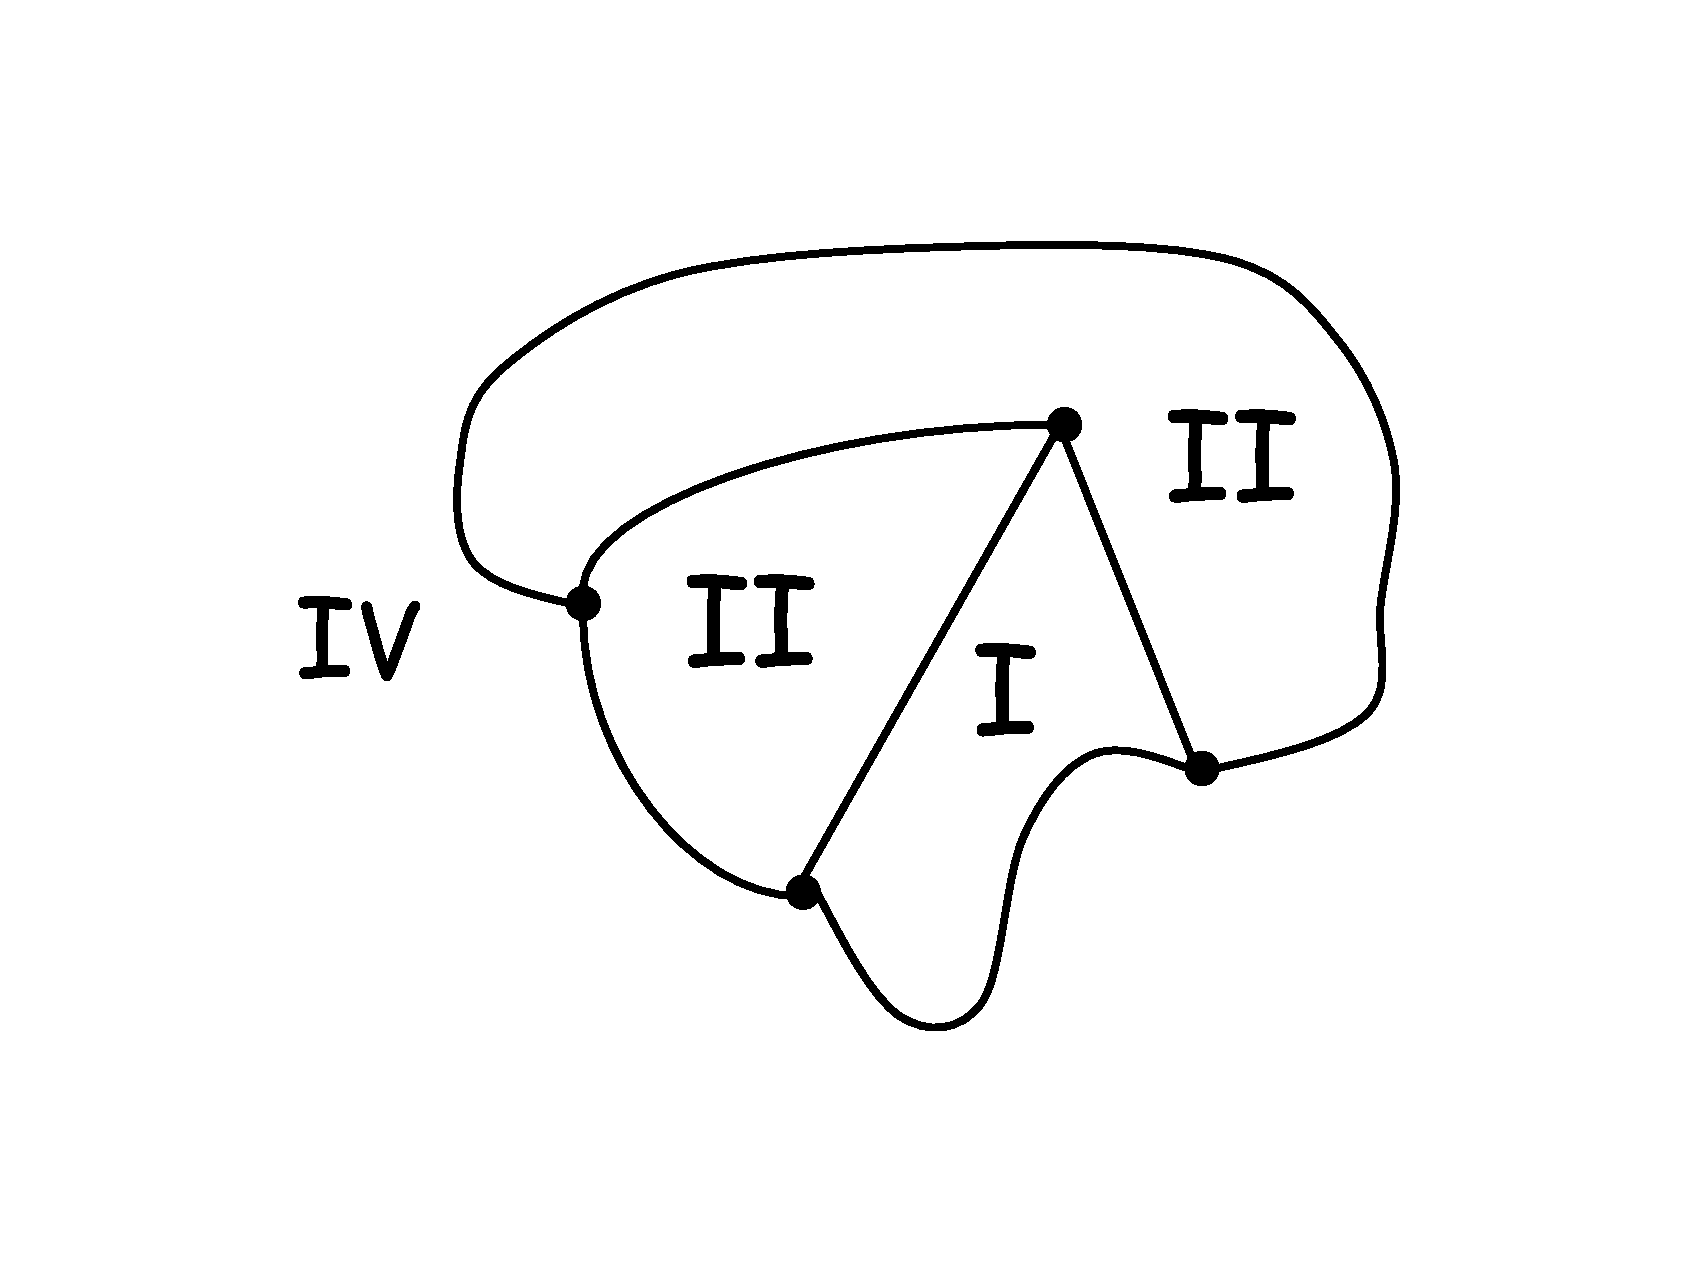
\includegraphics[height=2in]{continuous-faces}
\caption{A Planar Drawing with Four Faces.}
\label{fig:continuous-faces}
\end{figure}
Face IV, which extends off to infinity in all directions, is called the
\term{outside face}.

This definition of planar graphs is perfectly precise, but completely
unsatisfying: it invokes smooth curves and continuous regions of the plane
to define a property of a discrete data type.  So the first thing we'd
like to find is a discrete data type that represents planar drawings.

The clue to how to do this is to notice that the vertices along the
boundary of each of the faces in Figure~\ref{fig:continuous-faces} form a
simple cycle.  For example, labeling the vertices as in
Figure~\ref{fig:continuous-cycles}, the simple cycles for the face
boundaries are
\[
\mathtt{abca}\qquad \mathtt{abda}\qquad \mathtt{bcdb}\qquad \mathtt{acda}.
\]
Since every edge in the drawing appears on the boundaries of exactly two
continuous faces, every edge of the simple graph appears on exactly two of
the simple cycles.

\begin{figure}
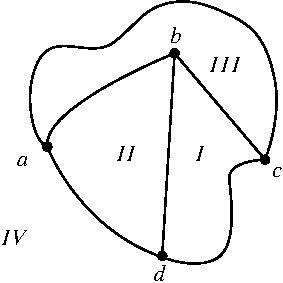
\includegraphics[height=2in]{continuous-cycles}
\caption{The Drawing with Labelled Vertices.}
\label{fig:continuous-cycles}
\end{figure}

Vertices around the boundaries of states and countries in an ordinary map
are always simple cycles, but oceans are slightly messier.  The ocean
boundary is the set of all boundaries of islands and continents in the
ocean; it is a \emph{set} of simple cycles (this can happen for countries
too ---like Bangladesh).  But this happens because islands (and the two
parts of Bangladesh) are not connected to each other.  So we can dispose
of this complication by treating each connected component separately.

But general planar graphs, even when they are connected, may be a bit more
complicated than maps.  For example a planar graph may have a
``\idx{bridge},'' as in Figure~\ref{fig:bridge}.
\begin{figure}[h]
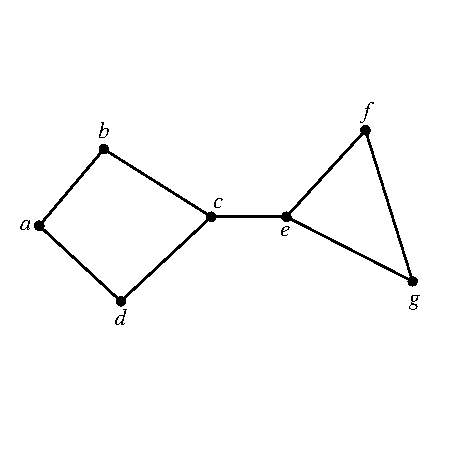
\includegraphics[height=2in]{edge-twice-same-face}
\caption{A Planar Drawing with a \emph{Bridge}.}
\label{fig:bridge}
\end{figure}
Now the cycle around the outer face is
\[
\mathtt{abcefgecda}.
\]
This is not a simple cycle, since it has to traverse the bridge
$\edge{c}{e}$ twice.

Planar graphs may also have ``\idx{dongles},'' as in
Figure~\ref{fig:dongle}.
\begin{figure}[h]
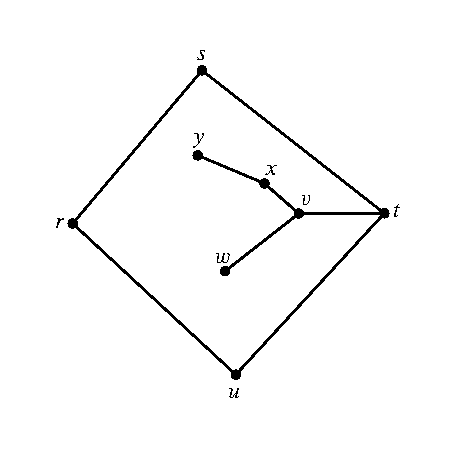
\includegraphics[height=2in]{dongle-face}
\caption{A Planar Drawing with a \emph{Dongle}.}
\label{fig:dongle}
\end{figure}
Now the cycle around the inner face is
\[
\mathtt{rstvxyxvwvtur},
\]
because it has to traverse \emph{every} edge of the dongle twice ---once
``coming'' and once ``going.''

But bridges and dongles are really the only complications, which leads
us to the discrete data type of \term{planar embeddings} that we can use
in place of continuous planar drawings.  Namely, we'll define a planar
embedding recursively to be the set of boundary-tracing cycles we could
get drawing one edge after another.

\iffalse  FAILED ATTEMPT TO AVOID RECURSIVE DEF
One property of the set of boundary-tracing cycles is that every
edge is traversed a total of two times by cycles in the set.  This is
almost enough to pin down exactly when a set of cycles are the
boundary-tracing cycles of a planar drawing, but not quite.  To illustrate
the remaining technicality, look at Figure~\ref{fig:bridge} showing a
bridge.  This graph has three faces described by the boundary-tracing
cycles
\[
\mathtt{abcefgecda} \text{ (the outer face)} \qquad \mathtt{abcda}\qquad
\mathtt{efge}.
\]
But we might also split up the cycle for the outer boundary into two
cycles, giving the set of four cycles,
\[
\mathtt{abcecda}\qquad \mathtt{efge} \qquad \mathtt{abcda}\qquad
\mathtt{efge}
\]
We don't want to allow this kind of splitting up of genuine
boundary-tracing cycles, but the four cycles above do have the property
that every edge is still traversed exactly twice.  What's wrong with the
split cycles is that they backtrack on themselves when they don't have to
---backtracks should only occur when there's nowhere else to go.  More
precisely:
\begin{definition}
A cycle in a graph has a \emph{backtrack} at vertex $v$ iff it contains a
subsequence $w,v,w$ for some vertex, $w$.  A backtrack at $v$ is
\emph{necessary} iff $v$ has degree 1.
\end{definition}
Now we're finally ready to define planar embeddings.

Let $G$ be a connected graph.  A \emph{planar embedding} of $G$ is a
set\footnote{\label{C} There is one exception to this definition.  If $G$
is isomorphic to the simple cycle, $C_n$, then a planar drawing of $G$ has
an inner and an outer face with the \emph{same} simple cycle as the
boundary of both faces.  So we need to use two ``copies'' of this simple
cycle as the set of boundary cycles for this graph.  But since this is the
only situation in which two faces have the same boundary cycle, this
exception is better explained in a footnote than mentioned explicitly in
the definition.} of cycles called \emph{boundary cycles}, such that
every edge of $G$ is traversed either
\begin{itemize}
\item by exactly two boundary cycles that are simple cycles, or

\item twice by a single boundary cycle that only backtracks when
necessary.
\end{itemize}


we can eliminate having to reason about continuous faces by jumping
directly to what matters about a continuous face, namely, the sequence of
vertices on its boundary curves.  This sequence is an undirected cycle in
the graph.  We'll call such an undirected cycle a \emph{discrete face},
and refer to a graph along with its discrete faces as a \emph{planar
embedding} of the graph.

The simplest kind of discrete face comes from the boundary of a country in
a map drawing ---this would just be a simple cycle.  Also, since each edge
appears on a boundary between two countries, it is traversed a total of
two times by the set of discrete faces.

But maps of countries are only a special case of planar graph.  For
example, a tree can always be drawn in the plane.  Such a tree drawing
``divides'' the plane into just \emph{one} region whose ``boundary'' is
the points and curves in the drawing, and the cycle of successive vertices
around this boundary backtracks on itself at every leaf.  But still, every
edge in the tree is traversed exactly twice (coming and going) by the
boundary of the tree.  So a planar graph will always have a set of
discrete faces such that each edge of the graph is traversed a total of
two times by these faces.

It turns out, conversely, that if a graph has a set of discrete faces that
traverse each edge a total of two times, the graph is in fact planar.  The
idea behind this claim is to consider how the successive discrete faces
could be drawn in the plane one at a time, with each new face having all
its edges on the boundary of one of the regions created so far (and in the
right order) so it can be added without the need to cross another face.

\textbf{MORE NEEDED HERE.}

But the only way to really prove this requires working with continuous
faces and continuously connected planar regions, which we don't want to
get into.  So we'll just accept the following definition:

\begin{definition}
A \emph{planar embedding} of a graph, $G$, is a set of cycles of $G$ such
that every edge is traversed a total of two times by these cycles.  Each
cycle is called a \emph{face} of the embedding.  A graph is \emph{planar}
iff it has a planar embedding.
\end{definition}
\fi

\subsection{Planar Embeddings}

By thinking of the process of drawing a planar graph edge by edge, we can
give a useful recursive definition of planar embeddings.

\begin{definition}\label{embeddingdef}
A \term{planar embedding} of a \emph{connected} graph consists of a
nonempty set of cycles of the graph called the \term{discrete faces} of
the embedding.  Planar embeddings are defined recursively as follows:

\begin{itemize}

\item \textbf{Base case:} If $G$ is a graph consisting of a single vertex,
$v$, then a planar embedding of $G$ has one discrete face, namely the
length zero cycle, $v$.

\item \textbf{Constructor Case:} (split a face) Suppose $G$ is a
connected graph with a planar embedding, and suppose $a$ and $b$ are
distinct, nonadjacent vertices of $G$ that appear on some discrete face,
$\gamma$, of the planar embedding.  That is, $\gamma$ is a cycle of the form
\[
a \dots b \cdots a.
\]
Then the graph obtained by adding the edge $\edge{a}{b}$ to the edges of
$G$ has a planar embedding with the same discrete faces as $G$, except
that face $\gamma$ is replaced by the two discrete
faces\footnote{\label{C} There is one exception to this rule.  If $G$ is a
line graph beginning with $a$ and ending with $b$, then the cycles into
which $\gamma$ splits are actually the same.  That's because adding edge
$\edge{a}{b}$ creates a simple cycle graph, $C_n$, that divides the plane
into an ``inner'' and an ``outer'' region with the same border.  In order
to maintain the correspondence between continuous faces and discrete
faces, we have to allow two ``copies'' of this same cycle to count as
discrete faces.  But since this is the only situation in which two faces
are actually the same cycle, this exception is better explained in a
footnote than mentioned explicitly in the definition.}
\[
a\dots ba\quad \text{ and } \quad ab\cdots a,
\]
as illustrated in Figure~\ref{fig:face-splitting}.

\begin{figure}[h]
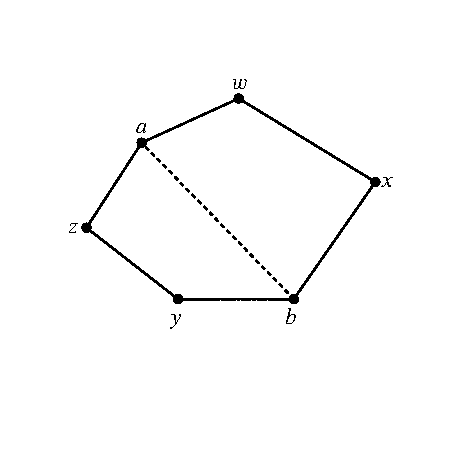
\includegraphics[height=2.5in]{split-a-face}
\caption{The Split a Face Case.}
\label{fig:face-splitting}
\end{figure}

\item \textbf{Constructor Case:} (add a bridge) Suppose $G$ and $H$ are
connected graphs with planar embeddings and disjoint sets of vertices.
Let $a$ be a vertex on a discrete face, $\gamma$, in the embedding of
$G$.  That is, $\gamma$ is of the form
\[
a\dots a.
\]
Similarly, let $b$ be a vertex on a discrete face, $\delta$, in the
embedding of $H$, so $\delta$ is of the form
\[
b\cdots b.
\]
Then the graph obtained by connecting $G$ and $H$ with a new edge,
$\edge{a}{b}$, has a planar embedding whose discrete faces are the union of
the discrete faces of $G$ and $H$, except that faces $\gamma$ and $\delta$
are replaced by one new face
\[
a\dots ab\cdots ba.
\]
This is illustrated in Figure~\ref{fig:add-bridge}, where the faces of
$G$ and $H$ are:
\[
G: \set{\texttt{axyza},\ \texttt{axya},\ \texttt{ayza}}
    \qquad H: \set{\texttt{btuvwb},\ \texttt{btvwb},\ \texttt{tuvt}},
\]
and after adding the bridge $\edge{\texttt{a}}{\texttt{b}}$, there is a
single connected graph with faces
\[
\set{\texttt{axyz{\color{blue}ab}tuvw{\color{blue}ba}},\
         \texttt{axya},\ \texttt{ayza},\ \texttt{btvwb},\ \texttt{tuvt}}.
\]
\begin{figure}[h]
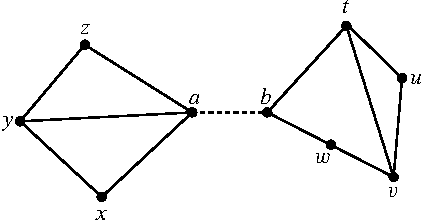
\includegraphics[height=3in]{add-bridge}
\caption{The Add Bridge Case.}
\label{fig:add-bridge}
\end{figure}

\end{itemize}

An arbitrary graph is \term{planar} iff each of its connected components
has a planar embedding.

\end{definition}

\subsection{What \idx{outer face}?}
Notice that the definition of planar embedding does not distinguish an
``outer'' face.  There really isn't any need to distinguish one.

In fact, a planar embedding could be drawn with any given face on the
outside.  An intuitive explanation of this is to think of drawing the
embedding on a \emph{sphere} instead of the plane.  Then any face can be
made the outside face by ``puncturing'' that face of the sphere,
stretching the puncture hole to a circle around the rest of the faces,
and flattening the circular drawing onto the plane.

So pictures that show different ``outside'' boundaries may actually be
illustrations of the same planar embedding.

This is what justifies the ``add bridge'' case in a planar embedding:
whatever face is chosen in the embeddings of each of the disjoint planar
graphs, we can draw a bridge between them without needing to cross any
other edges in the drawing, because we can assume the bridge connects
two ``outer'' faces.

\subsection{Euler's Formula}

The value of the recursive definition is that it provides a powerful
technique for proving properties of planar graphs, namely, structural
induction.

One of the most basic properties of a connected planar graph is that its
number of vertices and edges determines the number of faces in every
possible planar embedding:

\begin{theorem}[\idx{Euler's Formula}]
If a connected graph has a planar embedding, then
%
\[
v - e + f = 2
\]
%
where $v$ is the number of vertices, $e$ is the number of edges, and
$f$ is the number of faces.
\end{theorem}

For example, in Figure~\ref{fig:continuous-faces}, $\card{V} = 4$,
$\card{E} = 6$, and $f = 4$.  Sure enough, $4 - 6 + 4 = 2$, as Euler's
Formula claims.

\begin{proof}
The proof is by structural induction on the definition of planar
embeddings.  Let $P(\embed{E})$ be the proposition that $v - e + f = 2$ for an
embedding, $\embed{E}$.

\textbf{Base case:} ($\embed{E}$ is the one vertex planar embedding).
By definition, $v=1$, $e=0$, and $f=1$, so $P(\embed{E})$ indeed holds.

\textbf{Constructor case:} (split a face) Suppose $G$ is a connected graph
with a planar embedding, and suppose $a$ and $b$ are distinct, nonadjacent
vertices of $G$ that appear on some discrete face,
$\gamma= a \dots b \cdots a$, of the planar embedding.

Then the graph obtained by adding the edge $\edge{a}{b}$ to the edges of
$G$ has a planar embedding with one more face and one more edge than $G$.
So the quantity $v-e+f$ will remain the same for both graphs, and since by
structural induction this quantity is 2 for $G$'s embedding, it's also 2
for the embedding of $G$ with the added edge.  So $P$ holds for the
constructed embedding.

\textbf{Constructor case:} (add bridge) Suppose $G$ and $H$ are connected
graphs with planar embeddings and disjoint sets of vertices.  Then
connecting these two graphs with a bridge merges the two bridged faces
into a single face, and leaves all other faces unchanged.  So the bridge
operation yields a planar embedding of a connected graph with $v_G +v_H$
vertices, $e_G + e_H +1$ edges, and $f_G + f_H - 1$ faces.  But
\begin{align*}
\lefteqn{(v_G +v_H) - (e_G + e_H +1) + (f_G + f_H - 1)}\\
   & = (v_G  - e_G + f_G) + (v_H  - e_H  + f_H) -2\\
   & = (2)+(2)-2 & \text{(by structural induction hypothesis)}\\
   & = 2.
\end{align*}
So $v-e+f$ remains equal to 2 for the constructed embedding.  That is, $P$
also holds in this case.

This completes the proof of the constructor cases, and the theorem follows
by structural induction.
\end{proof}

\iffalse
\mfigure{!}{1in}{planar-assumptions}
\fi

\subsection{Number of Edges versus Vertices}

Like Euler's formula, the following lemmas follow by structural induction
directly from the definition of planar embedding.

\begin{lemma}\label{2e}
In a planar embedding of a connected graph, each edge is traversed once by
each of two different faces, or is traversed exactly twice by one face.
\end{lemma}

\begin{lemma}\label{3f}
  In a planar embedding of a connected graph with at least three vertices,
  each face is of length at least three.
\end{lemma}

\begin{corollary}\label{e3v}
Suppose a connected planar graph has $v \geq 3$ vertices and $e$ edges.
Then
\[
e \leq 3v-6.
\]
\end{corollary}

\begin{proof}
By definition, a connected graph is planar iff it has a planar embedding.
So suppose a connected graph with $v$ vertices and $e$ edges has a planar
embedding with $f$ faces.  By Lemma~\ref{2e}, every edge is traversed
exactly twice by the face boundaries.  So the sum of the lengths of the
face boundaries is exactly $2e$.  Also by Lemma~\ref{3f}, when $v \geq 3$,
each face boundary is of length at least three, so this sum is at least
$3f$.  This implies that
\begin{equation}\label{e3f}
3f \leq 2e.
\end{equation}
But $f = e-v+2$ by Euler's formula, and substituting into~\eqref{e3f} gives
\begin{align*}
3(e-v+2) & \leq 2e\\
e-3v + 6  & \leq 0\\
e & \leq 3v - 6
\end{align*}
\end{proof}

Corollary~\ref{e3v} lets us prove that the quadapi can't all shake hands
without crossing.  Representing quadapi by vertices and the necessary
handshakes by edges, we get the complete graph, \idx{$K_5$}.  Shaking
hands without crossing amounts to showing that $K_5$ is planar.  But $K_5$
is connected, has 5 vertices and 10 edges, and $10 > 3 \cdot 5-6$.  This
violates the condition of Corollary~\ref{e3v} required for $K_5$ to be
planar, which proves

\begin{lemma}\label{k5not}
$K_5$ is not planar.
\end{lemma}

Another consequence is
\begin{lemma}\label{d5}
Every planar graph has a vertex of degree at most five.
\end{lemma}

\begin{proof}
  If every vertex had degree at least 6, then the sum of the vertex
  degrees is at least $6v$, but since the sum equals $2e$, we have $e \geq
  3v$ contradicting the fact that $e \leq 3v-6 < 3v$ by
  Corollary~\ref{e3v}.
\end{proof}

\subsection{Planar Subgraphs}

If you draw a graph in the plane by repeatedly adding edges that don't
cross, you clearly could add the edges in any other order and still wind
up with the same drawing.  This is so basic that we might presume that our
recursively defined planar embeddings have this property.  But that
wouldn't be fair: we really need to prove it.  After all, the recursive
definition of planar embedding was pretty technical ---maybe we got it a
little bit wrong, with the result that our embeddings don't have this basic
draw-in-any-order property.

Now any ordering of edges can be obtained just by repeatedly switching the
order of successive edges, and if you think about the recursive definition
of embedding for a minute, you should realize that you can switch
\emph{any} pair of successive edges if you can just switch the last two.
So it all comes down to the following lemma.

\hyperdef{switch}{edges}{\begin{lemma}}\label{switch-edges} Suppose that,
  starting from some embeddings of planar graphs with disjoint sets of
  vertices, it is possible by two successive applications of constructor
  operations to add edges $e$ and then $f$ to obtain a planar embedding,
  $\embed{F}$.  Then starting from the same embeddings, it is also
  possible to obtain $\embed{F}$ by adding $f$ and then $e$ with two
  successive applications of constructor operations.
\end{lemma}

We'll leave the proof of Lemma~\ref{switch-edges} to
Problem~\ref{PS_planar_graph_construction_order}.

\begin{corollary}\label{permute-edges} Suppose that, starting from some
  embeddings of planar graphs with disjoint sets of vertices, it is
  possible to add a sequence of edges $e_0,e_1,\dots,e_n$ by successive
  applications of constructor operations to obtain a planar embedding,
  $\embed{F}$.  Then starting from the same embeddings, it is also
  possible to obtain $\embed{F}$ by applications of constructor operations
  that successively add any permutation\footnote{If $\pi:\set{0,1,\dots,n} \to
    \set{0,1,\dots,n}$ is a bijection, then the sequence
    $e_{\pi(0)},e_{\pi(1)},\dots,e_{\pi(n)}$ is called a \term{permutation} of
    the sequence $e_0,e_1,\dots,e_n$.} of the edges $e_0,e_1,\dots,e_n$.
\end{corollary}

\begin{corollary}\label{delete-edge}
Deleting an edge from a planar graph leaves a planar graph.

\begin{proof}
  By Corollary~\ref{permute-edges}, we may assume the deleted edge was the
  last one added in constructing an embedding of the graph.  So the
  embedding to which this last edge was added must be an embedding of the
  graph without that edge.
\end{proof}

\end{corollary}

Since we can delete a vertex by deleting all its incident edges,
Corollary~\ref{delete-edge} immediately implies

\begin{corollary}\label{delete-vertex}
Deleting a vertex from a planar graph, along with all its incident
edges of course, leaves another planar graph.
\end{corollary}

A \term{subgraph} of a graph, $G$, is any graph whose set of vertices is a
subset of the vertices of $G$ and whose set of edges is a subset of the
set of edges of $G$.  So we can summarize Corollaries~\ref{delete-edge}
and~\ref{delete-vertex} and their consequences in a Theorem.

\begin{theorem}\label{planar-subgraph}
  Any \index{planar subgraph}subgraph of a planar graph is planar.
\end{theorem}

\subsection{Planar \idx{5-Colorability}}

We need to know one more property of planar graphs in order to prove that
planar graphs are 5-colorable.

\begin{lemma}\label{mergelem}
Merging two adjacent vertices of a planar graph leaves another planar graph.
\end{lemma}

Here merging two adjacent vertices, $n_1$ and $n_2$ of a graph means
deleting the two vertices and then replacing them by a new ``merged''
vertex, $m$, adjacent to all the vertices that were adjacent to either of
$n_1$ or $n_2$, as illustrated in Figure~\ref{fig:merged}.

\begin{figure}%[h]
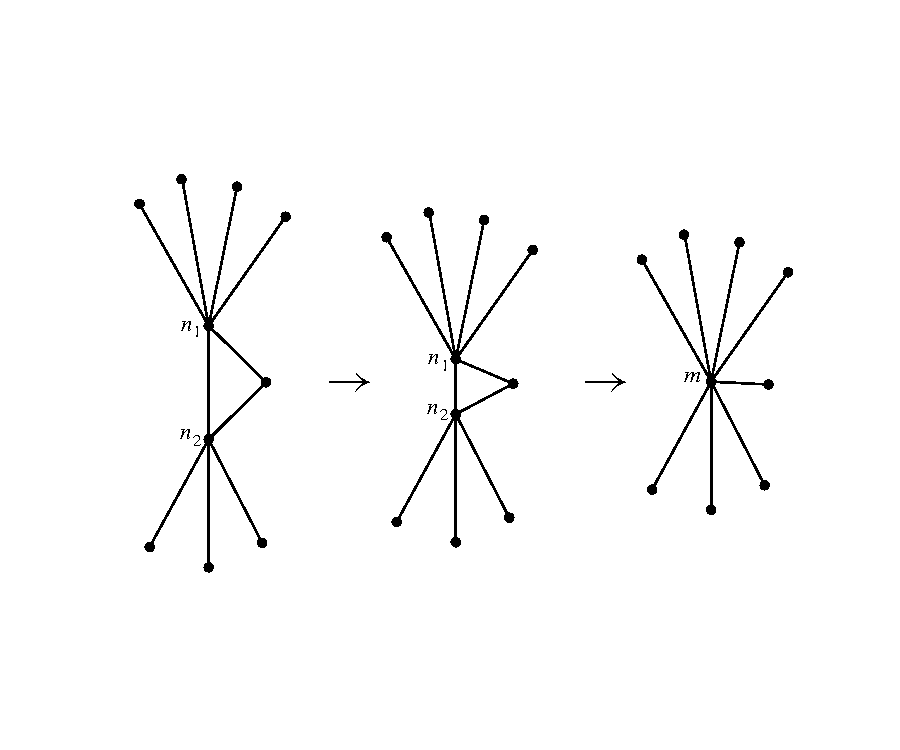
\includegraphics[height=4in]{vertex-merge-arrows}
\caption{Merging adjacent vertices $n_1$ and $n_2$ into new vertex, $m$.}
\label{fig:merged}
\end{figure}

Lemma~\ref{mergelem} can be proved by structural induction, but the proof
is kind of boring, and we hope you'll be relieved that we're going to omit
it.  (If you insist, we can add it to the next problem set.)

Now we've got all the simple facts we need to prove 5-colorability.
\begin{theorem}
Every planar graph is five-colorable.
\end{theorem}

\begin{proof}
The proof will be by strong induction on the number, $v$, of vertices, with
induction hypothesis:
\begin{quote}
Every planar graph with $v$ vertices is five-colorable.
\end{quote}

\textbf{Base cases} ($v \leq 5$): immediate.

\textbf{Inductive case}: Suppose $G$ is a planar graph with $v+1$
vertices.  We will describe a five-coloring of $G$.

First, choose a vertex, $g$, of $G$ with degree at most 5; Lemma~\ref{d5}
guarantees there will be such a vertex.

\textbf{Case 1} ($\degr{g}<5$): Deleting $g$ from $G$ leaves a graph, $H$,
that is planar by Lemma~\ref{delete-vertex}, and, since $H$ has $v$ vertices,
it is five-colorable by induction hypothesis.  Now define a five coloring
of $G$ as follows: use the five-coloring of $H$ for all the vertices besides
$g$, and assign one of the five colors to $g$ that is not the same as the
color assigned to any of its neighbors.  Since there are fewer than 5
neighbors, there will always be such a color available for $g$.

\textbf{Case 2} ($\degr{g}=5$): If the five neighbors of $g$ in $G$ were
all adjacent to each other, then these five vertices would form a
nonplanar subgraph isomorphic to $K_5$, contradicting
Theorem~\ref{planar-subgraph}.  So there must be two neighbors, $n_1$ and
$n_2$, of $g$ that are not adjacent.  Now merge $n_1$ and $g$ into a new
vertex, $m$, as in Figure~\ref{fig:merged}.  In this new graph, $n_2$ is
adjacent to $m$, and the graph is planar by Lemma~\ref{mergelem}.  So we
can then merge $m$ and $n_2$ into a another new vertex, $m'$, resulting in
a new graph, $G'$, which by Lemma~\ref{mergelem} is also planar.  Now $G'$
has $v-1$ vertices and so is five-colorable by the induction hypothesis.

Now define a five coloring of $G$ as follows: use the five-coloring of $G'$
for all the vertices besides $g$, $n_1$ and $n_2$.  Next assign the color
of $m'$ in $G'$ to be the color of the neighbors $n_1$ and $n_2$.  Since
$n_1$ and $n_2$ are not adjacent in $G$, this defines a proper
five-coloring of $G$ except for vertex $g$.  But since these two neighbors
of $g$ have the same color, the neighbors of $g$ have been colored using
fewer than five colors altogether.  So complete the five-coloring of $G$ by
assigning one of the five colors to $g$ that is not the same as any of the
colors assigned to its neighbors.

\end{proof}

A graph obtained from a graph, $G$, be repeatedly deleting vertices,
deleting edges, and merging adjacent vertices is called a \term{minor} of
$G$.  Since \idx{$K_5$} and \idx{$K_{3,3}$} are not planar,
Lemmas~\ref{delete-edge},~\ref{delete-vertex}, and~\ref{mergelem}
immediately imply:

\begin{corollary}\label{forbiddenK}
  A graph which has $K_5$ or $K_{3,3}$ as a minor is not planar.
\end{corollary}

We don't have time to prove it, but the converse of
Corollary~\ref{forbiddenK} is also true.  This gives the following famous,
very elegant, and purely discrete characterization of planar graphs:

\begin{theorem}[\idx{Kuratowksi}]
  A graph is not planar iff it has $K_5$ or $K_{3,3}$ as a minor.
\end{theorem}

\subsection{Classifying \idx{Polyhedra}}

The \idx{Pythagoreans} had two great mathematical secrets, the
irrationality of $\sqrt{2}$ and a geometric construct that we're about to
rediscover!

A \term{polyhedron} is a convex, three-dimensional region bounded by a
finite number of polygonal faces.  If the faces are identical regular
polygons and an equal number of polygons meet at each corner, then the
polyhedron is \index{regular polyhedron}\term*{regular}.  Three examples
of regular polyhedra are shown below: the tetrahedron, the cube, and the
octahedron.

\mfigure{!}{1.25in}{polyhedra}

We can determine how many more regular polyhedra there are by thinking
about planarity.  Suppose we took \emph{any} polyhedron and placed a
sphere inside it.  Then we could project the polyhedron face boundaries
onto the sphere, which would give an image that was a planar graph
embedded on the sphere, with the images of the corners of the polyhedron
corresponding to vertices of the graph.  But we've already observed that
embeddings on a sphere are the same as embeddings on the plane, so Euler's
formula for planar graphs can help guide our search for regular polyhedra.

For example, planar embeddings of the three polyhedra above look like
this:

%\mfigure{!}{1.25in}{polyhedra-blowup}
\begin{center}
\setlength{\unitlength}{2000sp}%{3947sp}%
%
\begingroup\makeatletter\ifx\SetFigFont\undefined%
\gdef\SetFigFont#1#2#3#4#5{%
  \reset@font\fontsize{#1}{#2pt}%
  \fontfamily{#3}\fontseries{#4}\fontshape{#5}%
  \selectfont}%
\fi\endgroup%
\begin{picture}(9999,2124)(1489,-3073)
%\thinlines
{\color[rgb]{0,0,0}\put(8476,-3061){\line( 3, 4){1548}}
\put(9976,-961){\line( 3,-4){1548}}
\put(11476,-3061){\line(-1, 0){3000}}
}%
{\color[rgb]{0,0,0}\put(9526,-2011){\line( 1, 0){900}}
\put(10426,-2011){\line(-3,-5){450}}
\put(9976,-2761){\line(-3, 5){450}}
}%
{\color[rgb]{0,0,0}\put(8476,-3061){\line( 1, 1){1050}}
\put(9526,-2011){\line( 2, 5){424.138}}
}%
{\color[rgb]{0,0,0}\put(9976,-961){\line( 2,-5){424.138}}
\put(10426,-2011){\line( 1,-1){1050}}
}%
{\color[rgb]{0,0,0}\put(11476,-3061){\line(-5, 1){1500}}
\put(9976,-2761){\line(-5,-1){1500}}
}%
{\color[rgb]{0,0,0}\put(3001,-1261){\line(-5,-6){1500}}
\put(1501,-3061){\line( 1, 0){3000}}
\put(4501,-3061){\line(-5, 6){1500}}
\put(3001,-1261){\line( 0,-1){1200}}
\put(3001,-2461){\line(-5,-2){1500}}
}%
{\color[rgb]{0,0,0}\put(3001,-2461){\line( 5,-2){1500}}
}%
{\color[rgb]{0,0,0}\put(5401,-3061){\framebox(2100,2100){}}
}%
{\color[rgb]{0,0,0}\put(6001,-2461){\framebox(900,900){}}
}%
{\color[rgb]{0,0,0}\put(5401,-961){\line( 1,-1){600}}
}%
{\color[rgb]{0,0,0}\put(5401,-3061){\line( 1, 1){600}}
}%
{\color[rgb]{0,0,0}\put(7501,-3061){\line(-1, 1){600}}
}%
{\color[rgb]{0,0,0}\put(7501,-961){\line(-1,-1){600}}
}%
\end{picture}%

\end{center}

Let $m$ be the number of faces that meet at each corner of a
polyhedron, and let $n$ be the number of sides on each face.  In the
corresponding planar graph, there are $m$ edges incident to each of
the $v$ vertices.  Since each edge is incident to two vertices, we
know:
%
\[
m v = 2 e
\]
%
Also, each face is bounded by $n$ edges.  Since each edge is on the
boundary of two faces, we have:
%
\[
n f = 2 e
\]
%
Solving for $v$ and $f$ in these equations and then substituting into
\idx{Euler's formula} gives:
\[
\frac{2e}{m} - e + \frac{2e}{n} = 2
\]
which simplifies to
\begin{equation}\label{1m1n}
\frac{1}{m} + \frac{1}{n} = \frac{1}{e} + \frac{1}{2}
\end{equation}
%
This last equation~\eqref{1m1n} places strong restrictions on the
structure of a polyhedron.  Every nondegenerate polygon has at least 3
sides, so $n \geq 3$.  And at least 3 polygons must meet to form a corner,
so $m \geq 3$.  On the other hand, if either $n$ or $m$ were 6 or more,
then the left side of the equation could be at most $1/3 + 1/6 = 1/2$,
which is less than the right side.  Checking the finitely-many cases that
remain turns up only five solutions.  For each valid combination of $n$
and $m$, we can compute the associated number of vertices $v$, edges $e$,
and faces $f$.  And polyhedra with these properties do actually exist:
%
\[
\begin{array}{cc|ccc|l}
n & m & v  & e  &  f & \text{polyhedron} \\ \hline
3 & 3 & 4  & 6  &  4 & \text{tetrahedron} \\
4 & 3 & 8  & 12 &  6 & \text{cube} \\
3 & 4 & 6  & 12 &  8 & \text{octahedron} \\
3 & 5 & 12 & 30 & 20 & \text{icosahedron} \\
5 & 3 & 20 & 30 & 12 & \text{dodecahedron}
\end{array}
\]
%
The last polyhedron in this list, the dodecahedron, was the other great
mathematical secret of the Pythagorean sect.  These five, then, are the
only possible regular polyhedra.

So if you want to put more than 20 geocentric satellites in orbit so that
they \emph{uniformly} blanket the globe ---tough luck!

%% Planar Graphs Problems %%%%%%%%%%%%%%%%%%%%%%%%%%%%%%%%%%%%%%%%%%%%%%%%%%%%%
\begin{problems}

\examproblems
\pinput{MQ_planar_isomorphism}

\classproblems
\pinput{CP_planar_embedding_isomorphism}
\pinput{CP_K33_not_planar}
\pinput{CP_planar_structural_induction}

\homeworkproblems
\pinput{PS_triangle_free_planar_graphs}
\pinput{PS_planar_graph_construction_order}

%\pinput{CP0506_}
\end{problems}

%% Conclusion %%%%%%%%%%%%%%%%%%%%%%%%%%%%%%%%%%%%%%%%%%%%%%%%%%%%%%%%%%%%%%%%%
%\TBA{Add conclusion here...}

\endinput


%% Conclusion %%%%%%%%%%%%%%%%%%%%%%%%%%%%%%%%%%%%%%%%%%%%%%%%%%%%%%%%%%%%%%%%%
%\TBA{Add conclusion here...}

\endinput
